%\documentclass[11pt, a4paper]{article}
\documentclass[]{vgtuef}
%\usepackage[left=25mm,right=15mm,top=15mm,bottom=15mm]{geometry}
\usepackage[utf8x]{inputenc}
\usepackage[L7x]{fontenc}
\usepackage[lithuanian]{babel}
\usepackage{url}
\usepackage{float}
\usepackage{graphicx}
\usepackage{amsmath}
\usepackage{fancyhdr}
\usepackage{datetime}
\graphicspath{{img/}}
\usepackage{tikz}
\usepackage{gensymb}
\usepackage{epstopdf}
\renewcommand{\baselinestretch}{1.5}
\usepackage{subfig} 
%\usepackage{lastpage}
\usepackage{pgfplots}
%\usepackage{afterpage}
\usetikzlibrary{arrows}

\begin{document}

  \begin{titlepage}
    \begin{center}
      
\includegraphics[width=70pt]{img/vgtu_logo.png}\\
      \textsc{\LARGE Vilniaus Gedimino Technikos universitetas}\\[1mm]
      \textsc{\Large Elektronikos fakultetas}\\[1mm]
      \textsc{\Large Elektroninių sistemų katedra}\\[40mm]
      \textsc{\Large Maksim NORKIN}\\[1mm]
      \textsc{\Large Objekto padėties nustatymas taikant MEMS jutiklius}\\[15mm]
      \textsc{\Large Investigation of the MEMS Sensor Based Object Position Estimation Methods}\\[10mm]
      \textsc{\large Magistro baigiamasis darbas}\\[10mm]
      \textsc{Informatikos inžinerijos studijų kryptis}\\
      \textsc{Informacinių elektroninių sistemų studijų programa, valst. kodas 621E15003}\\
      \textsc{Atvirojo kodo sistemų specializacija}\\
      \vfill
      {\large Vilnius, \the\year}
    \end{center}
  \end{titlepage}


  \begin{titlepage}
    \setcounter{page}{7}
    \thispagestyle{plain}
    \begin{center}
      \textsc{\Large Vilniaus Gedimino Technikos universitetas}\\
      \textsc{\Large Elektronikos fakultetas}\\
      \textsc{\Large Elektroninių sistemų katedra}\\[10mm]
      \hfill
      \begin{minipage}{.35\linewidth}
        \begin{flushleft}
          \uppercase{Tvirtinu}\\
          Katedos vedėjas\\[5mm]
          \makebox[1.8in]{\hrulefill}\\
          \scriptsize{\textit{(parašas)}}\\
          \normalsize{\the\year m. \makebox[0.45in]{\hrulefill} mėn. \makebox[0.15in]{\hrulefill} d.}\\
        \end{flushleft}
      \end{minipage}\\[10mm]
      \textsc{\Large Maksim NORKIN}\\[1mm]
      \textsc{\Large Objekto padėties nustatymas taikant MEMS jutiklius}\\[15mm]
      \textsc{\Large Investigation of the MEMS Sensor Based Object Position Estimation Methods}\\[10mm]
      \textsc{\large Magistro baigiamasis darbas}\\[10mm]
      \textsc{Informatikos inžinerijos studijų kryptis}\\
      \textsc{Informacinių elektroninių sistemų studijų programa, valst. kodas 621E15003}\\
      \textsc{Atvirojo kodo sistemų specializacija}\\
    \end{center}
    %\afterpage{\null\newpage}
  \end{titlepage}

  \setcounter{page}{8}

  % Anotacija
  Maksim NORKIN

Objekto padėties nustatymas taikant MEMS jutiklius. 
Magistro baigiamasis darbas informatikos inžinerijos laipsniui. 
Vilniaus Gedimino technikos universitetas.
Vilnius \the\year, TODO p. TODO iliustracijų, lentelių, bibliotekų, priedų.

Darbo tikslas yra sukurti objekto padėties nustatymo sistemą, taikant MEMS jutiklius ir mikrovaldiklį.
Pradžioje yra išnagrinėjami esami įgyvendinti funkcionalumai ir apibrėžiama, kokie šiuo metu yra taikomi sprendimai uždaviniui spręsti.
Atlikus analizę, sudarytas darbo planas išnagrinėti tris filtrus -- tiesinį (angl. \textit{linear}), išplėstinį (angl. \textit{extended}) ir sekamą (angl. \textit{unscented}) Kalman filtrus.
Išplėstas Kalman filtras industrijoje yra taikomas kaip standartas navigacinėse sistemose, sprendžiant netiesinio tipo uždavinius.
Visi trys filtrai buvo įgyvendinti ,,Matlab'' aplinkoje ir atliktas filtrų rezultatų palyginimas.
Buvo nustatyta -- blogiausiai netiesinį filtravimą atlieka tiesinis Kalman filtras, geriausiai - sekamas Kalman filtras.
Labai arti buvo išplėstas ir sekamas Kalman filtrai.
Po atliktos analizės sekamas Kalman filtras buvo įgyvendintas mikrovaldiklyje STM32.
  
  \newpage

  \tableofcontents

  \newpage

  \section*{Žymenys ir santrumpos}

  \input{section/zymenis_ir_santrympos.tex}

  \section*{ĮVADAS}
  \addcontentsline{toc}{section}{Įvadas}

  Užduoties tikslas yra sukurti programinį paketą \textit{Cortex-M4} pagrindu veikiančiai įrangai, kuri sugebėtų komunikuoti su \textit{MPU 9250} devynių ašių MEMS jutikliu ir atiduotu gautus duomenis į pagrindinį kompiuterį.
Pagrindinis kompiuteris elgiasi kaip duomenų priėmimo mazgas ir tolimesnis jų skirstytojas.
Kaip tolimesnis mazgas duomenų apdorojimui yra programa, kuri atlieka pirminį duomenų filtravimą ir pateikia gautus duomenis sistemos naudotojui tolimesnei analizei.

Kuriant programine įrangą yra tikslas pritaikyti atviro kodo licencija, kad būtų užkirstas kelias piktybiniam darbo išnaudojimui, bei apsisaugoti nuo bet kokių teisinių ir socialinių ginčų.
Įterptinių sistemų bendruomenėje programinės įrangos atžvilgiu vyrauja atviro kodo principas.
Dėl šios priežasties atliktam darbui norima pritaikyti kuo atviresnę licenciją, kad nebūtų jokių ribojimų kodo panaudojime.
Dėl tos pačios priežasties, labai paprastėja licencijos pritaikymo uždavinys.
Prieš pritaikant licenciją, reikia patikrinti ar naudojamos programinės įrangos licencija leidžia keisti prieš tai buvusią licenciją.
Kuomet yra pritaikyta labai atvira licencija, kuri visiškai neriboja licencijavimo pagrindus, tuomet pakeistai programinei įrangai licencija pritaikyti yra labai paprasta. 

  \section{MEMS jutikliai}

  Šiame skyriuje apžvelgti MEMS pagreičio ir giroskopo tipo jutikliai. 
Aptariama, kokie yra didžiausi jų privalumai ir trūkumai (didelis duomenų triukšmas ir būdai jiems kompensuoti ar mažinti).

\subsection{Giroskopas}

MEMS tipo jutiklis \cite{perlmutter2012high} yra gaminamas staklėmis iš silikono mikro-apdorojimo būdu, turi labai mažai dalių, o jo gamybos kaštai yra gana maži.

MEMS giroskopai yra veikiami \textit{Coriolio efekto}, kuris sako, jog turint koordinačių ašį, sukantis kampiniu greičiu $w$, objektas su mase $m$, kuris juda greičiu $v$, yra veikiamas jėgos

\begin{equation}
    F_c = -2m(w \times v)
\end{equation}

MEMS giroskopai susideda iš vibracinės kilmės elementų, kurie yra naudojami matuojant \textit{Coriolio} efektą. 
Egzistuoja labai daug vibracinių geometrijų, tarp kurių yra vibracinis ratas ir kamertono giroskopai. 
Paprasčiausia geometrija susideda iš vienos masės, kuri skirta vibruoti viena ašimi. 
Kai tik giroskopas yra pasukamas, įvedama antrinė vibracija statmenai pirminei ašiai dėl \textit{Coriolis} jėgos. 
Dėl to, kampinis greitis gali būti apskaičiuojamas, matuojant antrinį apsisukimą. 
Šiuo metu MEMS jutikliai negali pasiekti tokio tikslumo lygio, kokį siūlo optiniai jutikliai, tačiau yra tikimasi, kad ateityje MEMS jutikliai tikslumu nebus prastesni nei optiniai jutikliai.

MEMS jutikliai turi labai daug privalumų, palyginti su kitais jutikliais \cite{titterton2004strapdown}:

\begin{enumerate}
    \item mažas dydis;
    \item mažas svoris;
    \item patvari konstrukcija;
    \item mažos galios naudojimas;
    \item labai greitas paleidimo laikas;
    \item pigi gamyba, esant dideliam mastui;
    \item patikimi;
    \item reikalauja labai mažai priežiūros;
    \item gali būti naudojami sudėtingomis sąlygomis;
\end{enumerate}

\subsubsection{Nuolatinė dedamoji}

Vidutinis kampo pokyčio matavimas, palaikant visišką giroskopo ramybės būseną, yra laikomas nuolatine giroskopo dedamąja. 
Matuojama yra $\degree/h$. 
Nuolatinės dedamosios klaida $\epsilon$ yra apskaičiuojama integruojant ir priklauso nuo laiko $\theta(t) = \epsilon \cdot t$.

Klaida gali būti nustatyta, panaudojus labai ilgo laikotarpio vidutinę vertę, kuomet giroskopas yra paliktas visiškos ramybės būsenos ir nėra veikiamas jokių išorinių jėgų. 
Kai tik nuolatinė dedamoji yra žinoma, labai yra svarbu ją kompensuoti tikro matavimo metu.

\subsubsection{Atsitiktinis kampinis pokytis}

Jutiklio vertės matavimo metu yra galimas triukšmas, sukeliamas terminių ir mechaninių trukdžių, kurių dažnis yra žymiai didesnis už jutiklio vertės matavimo dažnį.
Tokių veiksnių rezultatas yra signalas, kuriame yra balto triukšmo. 
Tai yra paprasčiausia eilė skaičių, kurių vidurkis lygus nuliui.
Nėra jokios koreliacijos ir yra visiškai atsitiktiniai skaičiai. 
Tokiu būdu kiekvienas atsitiktinis skaičius yra tolygiai paskirstytas ir turi baigtinį $\sigma^2$ pasiskirstymą.

Net ir neišvedus formulės (detalus išvedimas yra pateikiamas \cite{woodman2007introduction}) galima teigti, jog triukšmas įveda ,,atsitiktinio vaikščiojimo'' (angl. \textit{random walk}) klaidą integraliniame signale, kuri yra nulinio vidurkio ir kurios variacija didėja nuo laiko pokyčio šaknies.
\begin{equation}
    \sigma_{\theta} (t) = \sigma \cdot \sqrt{ \delta t \cdot t}
\end{equation}
Čia $\sigma$ yra triukšmo signalo pokytis, $t$ yra visas jutiklio įverčio nuskaitymo periodas, o $\delta t$ yra laiko skirtumas tarp nuskaitymų.

Kadangi dominantis įvertis yra kaip triukšmas, lemiantis integralinį signalą, labai dažnai gamintojai nurodo gaminamo jutiklio atsitiktinį kampinį pokytį. Jis yra žymimas $\degree/\sqrt{h}$. 
Pavyzdžiui, jeigu jutiklis yra $0,3\degree / \sqrt{h}$, tai reiškia, jog po vienos valandos standartinės variacijos pozicijos orientacijos klaida sudarys $0,3\degree$, po dviejų valandų $\sqrt{2} * 0,3 = 0.42 \degree$.

\subsection{Nuolatinės dedamosios stabilumas}

Nuolatinė dedamoji MEMS giroskope keičiasi laikui bėgant dėl virpėjimo triukšmo elektronikos ir kituose įtaisuose, kurie potencialiai gali būti paveikti atsitiktinio virpėjimo. 
Virpėjimo triukšmas yra $1/f$ spektro, kurio efektai yra pastebimi elektroniniuose komponentuose, esant žemiems dažniams. 
Esant aukštiems dažniams virpėjimas yra uždengiamas balto triukšmo. 
Nuolatinės dedamosios nestabilumas, kuris kyla dėl virpėjimo, dažniausiai yra modeliuojamas kaip atsitiktinis kampinis pokytis.

Nuolatinės dedamosios stabilumo įvertis nurodo, kiek gali keistis per fiksuotą laiko tarpą. 
Dažniausiai imamas $100~s$ laiko rėžis, kuomet aplinka visiškai nesikeičia. 
Įvertis žymimas kaip $1\sigma$ ir matuojamas $\degree/h$ arba $\degree/s$, kai įranga yra labai netiksli. 
Nuolatinės dedamosios stabilumas yra modeliuojamas atsitiktinio vaikščiojimo procesu. 
Tai galima interpretuoti turint $B_t$ kaip dedamosios vertė laiku $t$, tuomet $1\sigma$ stabilumas $0,01\degree/h$ per 100 sekundžių reiškia, kad dedamoji laiku $t+100$ yra atsitiktinis skaičius, kurio vertė yra tikėtina $B_t$ su $0,01\degree/h$ variacija. 
Po tam tikro laiko, variacija sukuria atsitiktinį vaikščiojimą, kurio nuokrypis didėja per laiko vieneto šaknį. 
Dėl šitos priežasties nuolatinės dedamosios stabilumas yra žymimas kaip dedamosios atsitiktinis vaikščiojimo matas

\begin{equation}
    BRW (\degree / \sqrt{h}) = \frac{BS(\degree/h)}{\sqrt{t(h)}},
\end{equation}
kur $t$ yra nuolatinės dedamosios stabilumo laikas.

Praktikoje yra truputį kitaip. 
Jeigu stabilumas būtų modeliuojamas kaip atsitiktinis vaikščiojimas, tai integracinis įverčio skaičiavimas smarkiai padidintų klaidos įvertį. 
Dėl to, yra nutarta nustatyti rėžius, kuriuose yra nurodomas stabilumas.

\subsubsection{Temperatūros efektai}

Temperatūros svyravimai kyla dėl aplinkos temperatūros nepastovumo ir pačio jutiklio temperatūros nepastovumo. 
Tokie svyravimai natūraliai įtakoja ir nuolatinę dedamąja. 
Jie visiškai nėra nurodomi nuolatinės dedamosios klaidos skaičiavimuose.

Bet koks likutinis nuolatinės dedamosios įterpimas dėl temperatūros pokyčio smarkiai padidins įverčio klaidą ir klaida laikui bėgant didės.
Santykis MEMS jutikliuose tarp temperatūros ir klaidos yra netiesinis.
Dauguma inercinių matavimo sistemų turi savo viduje temperatūros daviklį, todėl matavimo klaidą galima kompensuoti tokiu būdu. 
Kai kurios matavimo sistemos siūlo automatinį klaidos taisymą.

\subsubsection{Kalibravimo klaidos}

Kalibravimo klaidų terminas susieja grupę klaidų šaltinių, kurie susideda iš santykio faktoriaus, lygiavimo ir giroskopų tiesiškumo. 
Tokio tipo klaidų galima pastebėti tik išoriškai veikiant jutiklį ir stebint nuolatinės dedamosios pokytį. 
Tai sukelia integracinio signalo netikslumų, prie kurių prisideda papildomi svyravimai, kurių dydis yra santykis tarp pokyčio ir vykdymo laiko. 
Dažniausiai tokio tipo klaidas galima išmatuoti ir jas kompensuoti.

% Akcelerometras

\subsection{Pagreičio jutiklis}

Mikro-staklių pagaminti silikoniniai pagreičio jutikliai naudoja tokius pačius principus, kaip ir mechaniniai ar kietieji jutikliai. 
Egzistuoja du pagrindiniai MEMS pagreičio jutiklių tipai. 
Pirmas tipas yra mechaniniai pagreičio jutikliai, kurie yra pagaminti iš silikono. 
Jie veikia lygiai tokiais pačiais principais, kaip ir mechaniniai jutikliai. 
Antras jutiklių tipas - kurie matuoja vibracijos pokyčius vibraciniam elemente, ko pasekoje yra stebimi įtampos pokyčiai.

Pagreičio MEMS jutiklių privalumai yra lygiai tokie patys, kaip ir MEMS giroskopinių jutiklių. 
Taip pat, pagrindinis tokių jutiklių minusas prieš kito gaminimo tipo jutiklius - mažas tikslumas. 

\subsubsection{Nuolatinė dedamoji}

Vertės dedamoji, pagreičio matavimo jutiklyje, yra skirtumas tarp matuojamos vertės ir realios vertės, matuojama $m/s^2$.
Pastovios dedamosios klaida $\epsilon$, po dvigubos integracijos, sukuria klaidą, kuri laikui bėgant didėja keturis kartus. 
Sukaupta klaida, priklausomai nuo pozicijos yra

\begin{equation}
    s(t) = \epsilon \cdot \frac{t^2}{2},
\end{equation}
kur $t$ yra integravimo laikas.

Yra galimybių vertinti dedamąją atliekant matavimus su duotu jutikliu labai ilgą laiką, kuriuo neveikia jokia išorinė jėga. 
Deja, visiškai izoliuoti jutiklio nėra galima, kadangi iškarto erdvėje pradeda veikti gravitacija, kuri veikia jutiklį, patiekdama savo nuolatinę dedamąja. 
To pasekoje, labai svarbu yra žinoti įrenginio pozicija žemės atžvilgiu, iš kurios pusės veikia gravitacinė jėga. Praktikoje tai yra pasiekiama naudojant kalibravimo procedūra, kurios metu įrenginys yra pritvirtinamas prie paviršiaus, kurio orientacija gali būti kontroliuojama labai tiksliai.

\subsubsection{Atsitiktinis pagreičio pokytis}

Pagreičio MEMS jutiklio išėjimo matavimai yra veikiami balto triukšmo. 
Kaip jau buvo paminėta giroskopo atsitiktinio kampo pokyčio poskyryje, balto triukšmo integracija sudaro sąlygas variacijai didėti proporcingai $\sqrt{t}$. 
To pasekoje, jutiklio išėjime yra stebimas atsitiktinis verčių vaikščiojimas, kuris vertinamas $m/s/\sqrt{h}$. Praleidžiant standartinės variacijos išvedimą, kuris yra aprašytas \cite{woodman2007introduction}, galima iškarto teigti, kad pagreičio jutiklio baltas triukšmas sukuria antro lygio atsitiktinį verčių vaikščiojimą pozicijoje, su vidurkiu, kuris lygus nuliui ir standartiniu nuokrypiu

\begin{equation}
    \sigma_{s}(t) \approx \sigma \cdot t^{3/2} \cdot \sqrt{\frac{\delta t}{3}},
\end{equation}
kuris didėja proporcingai nuo $t^{3/2}$. 
Čia $t$ yra visas matavimo laikas, $\delta t$ yra skirtumas tarp įverčio matavimo laikų.

\subsubsection{Vibraciniai triukšmai}

MEMS tipo pagreičio jutikliai yra veikiami vibracijos triukšmo, kuris sukelia nuolatinės dedamosios stabilumo klaidą per laiką. 
Tokie nukrypimai yra dažnai modeliuojami kaip nuolatinės dedamosios atsitiktiniai judėjimai, kaip jau buvo aprašyta giroskopo atveju. 
Naudojantis tokiu modeliu, vibracijos sukuria antro lygio atsitiktinio vaikščiojimo triukšmą pagreičiui, proporcingai $t^{3/2}$ ir trečio lygio atsitiktinį vaikščiojimą, kuris yra proporcingas $t^{5/2}$.

\subsubsection{Temperatūros efektai}

Kaip ir giroskopu atžvilgiu, temperatūros pokyčiai įtakoja vibracinius pokyčius, kas sukelia dedamosios nestabilumus išėjimo signale. 
Dedamosios santykis su temperatūra labai priklauso nuo įrangos, tačiau dažniausiai jis yra ne linijinis. 
Bet koks liekamasis nuolatinės dedamosios komponentas sukelia klaida, kuri didėja keturgubai bėgant laikui. 
Pagreičio jutiklio korekcijos dėl temperatūros kai kurie matavimo įrenginiai automatiškai kompensuoja.

\subsubsection{Kalibravimo klaidos}

Kalibravimo klaidos atsiranda kaip nuolatinės dedamosios klaidos. 
Jie pasirodo įverčiuose tik tuomet, kai jutiklis yra veikiamas kažkokio pagreičio jėgos. 
Taip pat verta stebėti gravitaciją, kadangi ji gali sukelti tokias laikinas klaidas ir tuomet, kai jutiklis yra pastovioje pozicijoje ir nėra veikiamas išorinės pagreičio jėgos.



  \section{Signalų filtrai}

  Šiame skyriuje apžvelgti pagrindiniai signalų filtravimo įrankiai, kurie yra plačiai naudojami inercinėse navigacinėse sistemose.

\subsection{\textit{Kalman} filtras}

    \textit{Kalman} filtras \cite{kalman1960new} yra vienas iš labiausiai naudojamų duomenų sujungimo algoritmų informacijos apdorojimo pramonės srityje \cite{faragher2012understanding}. 
    Pats žymiausias \textit{Kalman} filtro panaudojimas jo ankstyvoje stadijoje yra \textit{Apollo} navigaciniam kompiuteryje, kuris nugabeno \textit{Neil Armstrong} iki mėnulio ir svarbiausia -- atgal. 
    Šiais laikais, \textit{Kalman} filtrą galima rasti beveik kiekviename įrenginyje -- mobiliam telefone, kompiuteriniuose žaidimuose.

    \subsubsection{Diskretaus laiko \textit{Kalman} filtras}

    Tarkime, kad turime linijinę diskretaus laiko sistemą

    \begin{equation}
        x_k = F_{k-1}x_{k-1} + G_{k-1}u_{k-1} + w_{k-1}
    \end{equation}
    \begin{equation}
        y_k = H_k x_k + v_k
    \end{equation}

    Proceso triukšmai ${w_k}$ ir ${v_k}$ yra baltasis, nulinio vidurkio, be koreliacijos ir žinomos kovariacijos matricos

    \begin{equation}
    w_k \sim (0, Q_k)
    \end{equation}
    \begin{equation}
    v_k \sim (0, R_k)
    \end{equation}
    \begin{equation}
    E[w_k w_j^T] = Q_k \delta_{k-j}
    \end{equation}
    \begin{equation}
    E[v_k v_j^T] = R_k\delta_{k-j}
    \end{equation}
    \begin{equation}
    E[v_k w_j^T] = 0,
    \end{equation}

    kur $\delta_{k-j}$ yra Kroneckerio delta funkcija, $\delta_{k-j} = 1$, jeigu $k=j$ ir $\delta_{k-j} = 0$, kai $k \neq j$.
    Tikslas yra spėti $x_k$ būsena, remiantis žiniomis apie sistemos dinamikas ir turimu mėginiu, kuris yra triukšmingas ${y_k}$.
    Informacijos kiekis, kuris yra galimas spėjimui skiriasi nuo problemos, kuria yra norima išspręsti.
    Jeigu egzistuoja visi mėginiai, iki laiko $k$, kuriuos galima panaudoti $x_k$ spėjimui, galima suformuoti tolesnį spėjimą, kuri galima pažymėti kaip $\hat{x}_k^{+}$.
    Ženklas $+$ reikia, kad spėjimas yra tolimesnis.
    Vienas iš būdu kaip galima suformuoti tolimesnę būseną yra apskaičiuoti spėjamą $x_k$ vertę, kuri priklauso nuo turimų mėginių iki laiko $k$:

    \begin{equation}
        \hat{x}_k^{+} = E[x_k|y_1,y_2, \dots , y_k]
    \end{equation}

    Jeigu turimi visi matavimai prieš (ir neįtraukiant) laiką $k$ naudojimui, tuomet galima suformuluoti ankstesnį spėjimą, kuris yra žymimas kaip $\hat{x}_k^{-}$.
    Pagalbinis žymėjimas $-$, reiškia ankstesnį spėjimą.
    Vienas iš būdų suformuluoti ankstesnį spėjimą yra apskaičiuoti $x_k$ vertę, kuri priklauso nuo visų turimų matavimų prieš laiką $k$:

    \begin{equation}
        \hat{x}_k^{-} = E[x_k|y_1,y_2,\dots, y_{k-1}]
    \end{equation}

    Labai svarbu pažymėti, jog $\hat{x}^-_k$ ir $\hat{x}_k^{+}$ abu kartu yra spėjimai tokio pačio lygumo; jie abu yra $x_k$ spėjimai.
    Tačiau, $\hat{x}_k^-$ yra $x_k$ spėjimas prieš $y_k$ matavimą, o $\hat{x}_k^+$ yra spėjimas po to, kai $y_k$ matavimas yra atliktas.
    Natūraliai yra tikimąsi, jog $\hat{x}_k^+$ bus geresnis spėjimas už $\hat{x}_k^-$, kadangi tuo metu yra daugiau informacijos skaičiuojant $\hat{x}_k^+$:

    \begin{enumerate}
        \item $\hat{x}_k^-$ = $x_k$ spėjimas prieš mėginio gavimą laiku $k$
        \item $\hat{x}_k^+$ = $x_k$ spėjimas, po mėginio gavimo laiku $k$
    \end{enumerate}

    Jeigu egzistuoja mėginiai po laiko $k$, kuriuos galima naudoti $x_k$ spėjimui, tuomet galima suformuoti glotnesnį spėjimą.
    Vienas iš būdų suformuoti glotnesnį spėjimą yra apskaičiuoti tikėtiną $x_k$ vertę, kuri priklauso nuo visų turimų įverčių

    \begin{equation}
        \hat{x}_{k|k+N} = E[x_k|y_1,y_2,\dots,y_k,\dots, y_{k+N}],
    \end{equation}
    kur $N$ yra teigimas skaičius, kurio vertė priklauso nuo specifinės problemos, kuri yra sprendžiama.
    Jeigu galima rasti geriausią $x_k$ spėjimą daugiau negu vienu žingsniu greičiau už turimus mėginius, galima suformuluoti spėjamą būseną.

    \begin{equation}
        \hat{x}_{k|k-M} = E[x_k|y_1,y_2, \dots, y_{y-M}],
    \end{equation}
    kur $M$ yra teigiamas skaičius, kurio vertė priklauso nuo sprendžiamo uždavinio.

    Tolimesniam žymėjime bus pateiktas $\hat{x}_0^+$ įvertis, kuris parodys pradinį $x_0$ įvertinimą prieš bet kokius turimus mėginius.
    Pirmas mėginys yra gaunamas laiku $k=1$.
    Kadangi neegzistuoja jokie mėginiai, kuriuos galima panaudoti spėti $x_0$, yra logiška suformuoti $\hat{x}^+_0$ kaip pradinės būsenos $x_0$ tikėtiną įvertį:

    \begin{equation}
        \hat{x}_0^+ = E(x_0)
    \end{equation}

    Spėjimo klaidos kovariacijos matricai pažymėti bus panaudotas $P_k$ žymėjimas.
    $P_k^-$ žymi $\hat{x}_k^-$ įvertinimo klaidos kovariaciją, o $P_k^+$ žymi $\hat{x}_k^+$ įvertinimo klaidą.

    \begin{equation}
        P_k^- = E[(x_k - \hat{x}_k^-)(x_k - \hat{x}_k^-)^T]
    \end{equation}
    \begin{equation}
        P_k^+ = E[(x_k - \hat{x}_k^+)(x_k-\hat{x}_k^+)^T]
    \end{equation}

    Po to, kai yra apdorotas įvertis laike $(k-1)$, gaunamas $x_{k-1}$ įvertinimas (žymimas $\hat{x}_{k-1}^+$) ir įverčio kovariacijos matrica (žymima $P_{k-1}^+$).
    Kai ateina laikas $k$, prieš apdorojant įverčiui laike $k$, apskaičiuojame $x_k$ įvertį (žymima $\hat{x}_k^-$) ir įverčio klaidos kovariacijos matricą (žymima $P_k^-$).
    Tuomet yra apdorojamas gautas įvertis laike $k$ ir patobuliname įvertį $x_k$.
    Gautas galutinis įvertis $x_k$ yra žymimas $\hat{x}_k^+$, o jo kovariacijos matrica $P_k^+$.

    Spėjimo procesas pradedamas nuo $\hat{x}_0^+$, geriausiai žinomos pradinės $x_0$ būsenos.
    Turint $\hat{x}_0^+$, kaip apskaičiuoti $\hat{x}_1^-$?
    Reikia prilyginti $\hat{x}_1^- = E(x_1)$.
    Reikia pažymėti, jog $\hat{x}_0^+ = E(x_0)$, ir prisiminti, kad $x$ vidurkis kinta laike

    \begin{equation}
        \bar{x}_k = F_{k-1}\bar{x}_{k-1} + G_{k-1}u_{k-1}
    \end{equation}

    Tokiu atveju gaunama

    \begin{equation}
        \hat{x}_1^- = F_0\hat{x}_0^+ + G_0u_0
    \end{equation}

    Šita lygtis yra specifinė lygtis, kuri rodo kaip gauti $\bar{x}_1^-$ iš $\bar{x}_0^+$. Labiau bendrinant, gaunama lygtis

    \begin{equation}
        \hat{x}_k^- = F_{k-1}\bar{x}_{k-1}^+ + G_{k-1}u{k-1}
    \end{equation}

    Ir jinai yra vadinama $\bar{x}$ laiko atnaujinimo lygtis.
    Nuo laiko $(k-1)^+$ iki laiko $k^-$, būsenos įvertis kinta tokiu pačiu principu, kaip ir būsenos vidurkis.
    Neegzistuoja jokios papildomos informacijos, kuri leistu atnaujinti būseną tarp laiko $(k-1)^+$ ir $k^-$, todėl reikia tiesiog atnaujinti būsenos įvertį, remiantis sistemos dinaminėmis žiniomis.

    Toliau reikia apskaičiuoti laiko atnaujinimo $P$ lygtį.
    Pradedama nuo $P_0^+$, kuris žymi pradinės būsenos įverčio $x_0$ kovariaciją.
    Jeigu labai gerai yra žinoma apie pradinę sistemos būseną, tuomet $P_0^+ = 0$.
    Jeigu visiškai nėra aišku apie pradinę sistemos būseną, tuomet $P_0^+ = \inf$.
    Bendrai, $P_0^+$ parodo pradinės $x_0$ būsenos neužtikrintumą

    \begin{equation}
        P_0^+ = E[(x_0 - \hat{x}_0^+)(x_0 - \hat{x}_0^+)^T]
    \end{equation}

    Turint $P_0^+$, kaip apskaičiuoti $P_1^-$? Reikia prisiminti kaip linijinės diskretaus laiko būsenos kovariacija kinta su laiku ir gaunam

    \begin{equation}
        P_1^- = F_0 P_0^+F_0^T + Q_0
    \end{equation}

    Tai yra specifinė lygtis, o bendresnė lygtis atrodo taip

    \begin{equation}
        P_k^- = F_{k-1}P_{k-1}^+F_{k-1}^T + Q_{k-1},
    \end{equation}
    ir vadinama $P$ laiko atnaujinimo lygtimi.

    Aukščiau yra išvestos lygtis, kurios yra skirtos apskaičiuoti $\hat{x}$ ir $P$.
    Dabar reikalinga išvesti lygtis, kurios skirtos atnaujinti $\hat{x}$ ir $P$ po atlikto sistemos matavimo.
    Turint $\hat{x}_k^-$, kaip apskaičiuoti $\hat{x}_k^+$? Tiek $x_k^-$ ir $x_k^+$ yra $x_k$ įverčiai.
    Vienintelis skirtumas tarp $\hat{x}_k^-$ ir $\hat{x}_k^+$, kad $\hat{x}_k^+$ yra gaunamas turint mėginį $y_k$.
    Remiantis mažiausių kvadratų teorija, mėginys $y_k$ keičia $x$ konstantos spėjimą:

    \begin{equation}
        K_k = P_{k-1}H_k^T(H_kP_{k-1}H_k^T + R_k)^{-1} = P_kH_k^TR_k^-1
    \end{equation}
    \begin{equation}
        \bar{x}_k = \bar{x}_{k-1} + K_k(y_k - H_k\bar{x}_{k-1})
    \end{equation}
    \begin{equation}
        P_k = (I - K_kH_k)P_{k-1},
    \end{equation}
    kur $\bar{x}_{k-1}$ ir $P_{k-1}$ yra įvertinimas ir jo kovariacija prieš $y_k$ matavimą ir $\bar{x}_k$ ir $P_k$ yra įvertinimas ir jo kovariacija po $y_k$ matavimo.

    Atlikę porą pakeitimų, gauname

    \begin{equation}
        K_k = P_{k}^+H_k^TR_k^{-1}
    \end{equation}
    \begin{equation}
        \bar{x}_k^+ = \bar{x}_k^- + K_k(y_k - H_k\bar{x}_k^-)
    \end{equation}
    \begin{equation}
        P_k^+ = (I-K_kH_k)P_{k}^-
    \end{equation}

    Taip yra gaunamos lygtis, kurios yra naudojamos įverčiams $\bar{x}_k$ ir $P_k$ atnaujinti, po gauto mėginio.
    Matrica $K_k$ aukštesnėse lygtyse yra vadinama \textit{Kalman} augimu.

    \subsubsection{Pavyzdys}

    Geriau suprasti turimą teoriją, pateikiamas Niutono sistemos pavyzdys, kurioje nėra jokios triukšmo, su pozicija $r$, greičiu $v$ ir pastoviu pagreičiu $a$.
    Sistema galima apibūdinti kaip

    \begin{equation}
        \begin{bmatrix} \dot{r} \\ \dot{v} \\ \dot{a} \end{bmatrix} =
        \begin{bmatrix} 0 & 1 & 0 \\ 0 & 0 & 1 \\ 0 & 0 & 0 \end{bmatrix}
        \begin{bmatrix} r \\ v \\ a \end{bmatrix}
    \end{equation}
    \begin{equation}
        \dot{x} = Ax
    \end{equation}

    Diskretizuota sistemos versija (su diskretizacijos periodu $T$) yra užrašoma kaip\

    \begin{equation}
        x_{k+1} = Fx_k,
    \end{equation}
    kur $F$ yra duodamas kaip

    \begin{equation}
        F = exp(AT) = I + AT + \frac{(AT)^2}{2!} + \dots =
        \begin{bmatrix}
            0 & T & T^2/2 \\
            0 & 1 & T \\
            0 & 0 & 1
        \end{bmatrix}
    \end{equation}

    \textit{Kalman} filtras tokiai sistemai yra išreiškiamas

    \begin{equation}
        \bar{x}_k^- = F\bar{x}_{k-1}^+
    \end{equation}
    \begin{equation}
        P_k^- = FP_{k-1}^+ F^T + Q_{k-1} = FP_{k-1}^+ F^T
    \end{equation}

    Ką galima pastebėti, kad kovariacijos įverčio klaidos matrica didėja tarp laiko $(k-1)^+$ (laikas $(k-1)$, po kurio gautas įvertis yra apdorotas) ir $k^-$ (laikas $k$, prieš apdorojant gautą įvertį).
    Kadangi nėra gaunamas joks mėginys tarp laikų $(k-1)^+$ ir $k^-$, yra daug logikos, jog duota kovariacijos matrica didėja.
    Dabar galima įvesti triukšmą, kuris būtų mėginio gavimo triukšmas $\sigma^2$

    \begin{equation}
        y_k = H_kx_k + v_k = \begin{bmatrix} 1 & 0 & 0 \end{bmatrix} x_k + v_k
    \end{equation}
    \begin{equation}
        v_k ~ (0, R_k)
    \end{equation}
    \begin{equation}
        R_k = \sigma^2
    \end{equation}

    \textit{Kalman} augimas gaunamas kaip

    \begin{equation}
        K_k = P_k^-H_k^T(H_kP_k^-H_k^T+R_k)^{-1}
    \end{equation}

    Perrašius $P_k$ kaip trijų elementų vektorių

    \begin{equation}
        K_k = \begin{bmatrix} P_{k,11}^- \\ P_{k,12}^- \\ P_{k,13}^- \end{bmatrix} \frac{1}{P_{k,11}^- + \sigma^2}
    \end{equation}

    Tolimesnė kovariacija gaunama

    \begin{equation}
        P_k^+ = P_k^- - K_kH_kP_k^-
    \end{equation}

    Kai yra gaunamas naujas matavimas, yra natūraliai tikimąsi, jog būsenos spėjimas bus tikslesnis.
    Tai reiškia, jog kovariacija mažės, ką ir rodo lygtis.

    \subsection{Ištiesintas \textit{Kalman} filtras}

    Šiame skyriuje parodoma kaip ištiesinti ne tiesinę sistemą ir tuomet panaudoti \textit{Kalman} filtro teoriją įvertinant skirtumus tarp būsenos ir nominalios būsenos vertės.
    Toliau tai suteiks ne tiesinės sistemos būsenos įvertinimą.
    Ištiesintas \textit{Kalman} filtras yra išvedamas iš nuolatinio laiko požiūrio, o diskretaus ar hibridinio laiko išvedimai yra analogiški.

    Tarkime, egzistuoja toks ne tiesinės sistemos modelis:

    \begin{equation}
        \dot{x} = f(x,u,w,t)
    \end{equation}
    \begin{equation}
        y = h(x,v,t)
    \end{equation}
    \begin{equation}
        w ~ (0,Q)
    \end{equation}
    \begin{equation}
        v ~ (o,R)
    \end{equation}

    Sistemos lygtis $f(\cdot)$ ir matavimo lygtis $h(\cdot)$ yra ne tiesinės funkcijos.
    Bus naudojama Tailoro eilutė išplėsti šitas lygtis aplink nominalią kontrolę $u_0$ ir nominalią būseną $x_0$ su $y_0$ išėjimu, bei triukšmu $w_0$ir $v_0$.
    Šios nominalios vertės yra paremtos ankstesniu spėjimu apie sistemos trajektoriją.
    Pavyzdžiui, jeigu sistemos lygtis pateikia lėktuvo dinamikas, tuomet nominali kontrolė, būsena ir išėjimas gali būti suplanuoto skrydžio trajektorija.
    Reali skrydžio trajektorija skirsis nuo šios nominalios trajektorijos dėl modeliavimo klaidos, trikdymų ir kitų nenumatytų efektų.
    Tačiau reali trajektorija turi būti arti nominalios trajektorijos, tokiu atveju Tailoro eilutės tiesinimas turi būti labai arti.
    Tailoro eilutės išskleidimas suteikia

    \begin{equation}
        \begin{aligned}
            \dot{x} &\approx f(x_0, u_0, w_0, t) + \frac{\delta f}{\delta x}\Bigr|_{0} (x-x_0) + \frac{\delta f}{\delta u}\Bigr|_{0} (u-u_0) + \frac{\delta f}{\delta w}\Bigr|_{0} (w-w_0) \\
            &= f(x_0, u_0, w_0, t) + A\Delta x + B \Delta u + L \Delta w
        \end{aligned}
    \end{equation}
    \begin{equation}
        \begin{aligned}
            y &\approx h(x_0, v_0, t) + \frac{\delta h}{\delta x}\Bigr|_{0}(x-x_0) + \frac{\delta h}{\delta v}\Bigr|_{0}(v-v_0) \\
            &= h(x_0, v_0, t) + C \Delta x + M \Delta v
        \end{aligned}
    \end{equation}

    Šie dalinių matricų A, B, C, L ir M išvestinės yra išskiriamos iš aukštesnių lygčių.
    Indeksas "0" rodo, kad dalinę išvestinę reikia atlikti esant nominaliai kontrolei, būsenai, išėjimui ir triukšmams.

    Galima padaryti prielaida, kad nominalaus triukšmo įverčiai yra abu lygus 0 šiuo atveju.
    Kadangi jie abu yra lygus 0, tuomet $\delta w(t) = w(t)$ ir $\delta v(t) = v(t)$.
    Toliau galima teigti, kad kontrolė $u(t)$ yra labai gerai žinoma.
    Bendru atveju, tai yra labai gera prielaida, kadangi kontrolės įėjimas $u(t)$ yra pateiktas sistemos kontrolės, kuri neturi turėti jokių abejonių įverčiuose.
    Tai reiškia, kad $u_0(t) = u(t)$ ir $\delta u(t) = 0$.
    Tačiau, realybėje gali būti neužtikrintumas kontrolės išėjime, kadangi jos yra sujungtos su kažkokiu įtaisu, kuris turi savo vidurkį ir triukšmą.
    Dabar galima aprašyti nominalios sistemos trajektoriją kaip

    \begin{equation}
        \label{eq:nominal_sistem_trajektory}
        \begin{aligned}
            \dot{x}_0 &= f(x_0, u_0, w_0, t) \\
            y_0 &= h(x_0, v_0, t)
        \end{aligned}
    \end{equation}

    Aprašytas nukrypimas nuo tikros sistemos būsenos išvestinę iš nominalios būsenos išvestinės ir nukrypimas nuo realaus mėginio iš nominalaus mėginio

    \begin{equation}
        \Delta \dot{x} = \dot{x} - \dot{x}_0 \\
        \Delta y = y - y_0
    \end{equation}

    Su šitais apibrėžimais, lygtis tampa

    \begin{equation}
        \Delta \dot{x} = A \Delta x + Lw = A \Delta x \tilde{w}
    \end{equation}
    \begin{equation}
        \tilde{w} \sim (0, \tilde{Q}), \tilde{Q} = LQL^T
    \end{equation}
    \begin{equation}
        \Delta y = C \Delta x + Mv = C \Delta x + \tilde{v}
    \end{equation}
    \begin{equation}
        \tilde{v} \sim (O, \tilde{R}), \tilde{R} = MRM^T
    \end{equation}

    Ši lygtis yra tiesinė sistema su $\Delta x$ būsena ir $\Delta y$ mėginiu.
    Tokiu atveju galima panaudoti \textit{Kalman} filtrą spėti $\Delta x$.
    Filtro įėjimas susideda iš $\Delta y$, kuris yra skirtumas tarp realaus matavimo $y$ ir nominalaus matavimo $y_0$.
    \textit{Kalman} filtro išėjimas $\Delta x$ yra įvertinimas skirtumo tarp realios būsenos $x$ ir nominalios būsenos $x_0$.
    Filtro lygtis ištiesintai sistemai yra

    \begin{equation}
        \label{eq:linerialized_kalman_filter}
        \begin{aligned}
            \Delta \hat{x} (0) &= 0\\
            P(0) &= E[(\Delta x(0) - \Delta \hat{x}(0))(\Delta{x}(0) - \Delta \hat{x}(0))^T]\\
            \Delta \dot{\hat{x}} &= A \Delta \hat{x} \\
            K &= PC^T\tilde{R}^{-1}\\
            \dot{P} &= AP + PA^T + \tilde{Q} - PC^T\tilde{R}^{-1}CP\\
            \hat{x} &= x_0 + \Delta \hat{x}
        \end{aligned}
    \end{equation}

    \textit{Kalman} filtrui, $P$ yra kovariacijos matricos klaida.
    Ištiesintas \textit{Kalman} filtras nėra tikras filtras, dėl klaidų, kurias suteikia ištiesinimas.
    Tačiau, jeigu ištiesinimo klaidos yra mažos, $P$ turėtų būti apie spėjimo klaidos kovariacijos įvertį.


\subsection{Išplėstasis \textit{Kalman} filtras}

    Ankstesniam skyriuje buvo aptartas tiesinis \textit{Kalman} filtras, kuris yra naudojamas spėti ne tiesinės sistemos būseną.
    Išvedimas buvo paremtas ne tiesinės sistemos tiesinimu aplink nominalios būsenos trajektorijos pokytį.
    Klausimas kyla, kaip gi reikia nustatyti tą nominalę būsenos trajektoriją?
    Kai kuriais atvejais, tai nėra labai paprastas uždavinys.
    Tačiau, kadangi \textit{Kalman} filtras spėja sistemos būseną, galima panaudoti patį \textit{Kalman} filtrą, kaip tą sistemos trajektorijos nominalę.
    Tai yra šioks toks savikėlimo metodas.
    Tiesinam ne tiesinę sistemą aplink \textit{Kalman} filtro būsenos spėjimą, o \textit{Kalman} filtro įvertinimas paremtas tiesine sistema.
    Tai yra išplėstojo \textit{Kalman} filtro idėja, kuri buvo pasiūlyta Stanley Schmidt.
    Autorius norėjo pritaikyti \textit{Kalman} filtrą ne tiesinėms erdvėlaivio navigacijos problemoms spręsti.

\subsubsection{Nepertraukiamo laiko išplėstasis \textit{Kalman} filtras}

        Sujungiant \ref{eq:nominal_sistem_trajektory} ir \ref{eq:linerialized_kalman_filter} lygtis, gaunama

        \begin{equation}
            \dot{x}_0 + \delta \dot{\hat{x}} = f(x_0, u_0, w_0, t) + A \Delta \hat{x} + K[y-y_0 -C(\hat{x} - x_0)]
        \end{equation}

        Toliau reikia pasirinkti tokį $x_0(t)=\hat{x}(t)$, kad $\Delta\hat{x}(t) = 0$ ir $\Delta\hat{\bar{x}}(t) = 0$.
        Kitais žodžiais, tiesinimo trajektorija $x_0(t)$ yra lygi ištiesinto \textit{Kalman} filtro įverčiui $\hat{x}(t)$.
        Tuomet nominalaus įverčio išraiška tampa

        \begin{equation}
            y_0 = h(x_0, v_0, t) = h(\hat{x}, v_0, t)
        \end{equation}

        Tai yra ekvivalentu ištiesintam \textit{Kalman} filtrui, tačiau čia pasirinkta $x_0 = \hat{x}$ ir yra perskirstytos lygtis, kad tiesiogiai gauti $\hat{x}$.
        \textit{Kalman} padidėjimas yra toks pats, kaip ir ankščiau.
        Tačiau šita formuluotė naudoja mėginį $y$ tiesiogiai, ir išėjime būsenos įvertis $\hat{x}$ irgi yra pateikiamas tiesiogiai.
        Tai yra dažnai žymima kaip išplėstas Kalman-Bucy filtras, kadangi Ričardas Bucy bendradarbiavo su Rudolfu Kalman pirmoje publikacijoje apie nepertraukiamo laiko \textit{Kalman} filtrą.
        Nepertraukiamo laiko išplėstas \textit{Kalman} filtras gali būti suvestas į tokius punktus

        \begin{enumerate}
            \item Sistemos lygtis yra tokios
            \begin{equation}
                \begin{aligned}
                \bar{x} &= f(x, u, w, t) \\
                y &= h(x, v, t) \\
                w &\sim (0,Q) \\
                v &\sim (0, R)
                \end{aligned}
            \end{equation}
            \item Apskaičiuoti duotas dalines išvestinių matricas kaip dabartinės būsenos įvertinimus
            \begin{equation}
                \begin{aligned}
                    A &= \frac{\delta f}{\delta x}\Bigr|_{\hat{x}} \\
                    L &= \frac{\delta f}{\delta w}\Bigr|_{\hat{x}} \\
                    C &= \frac{\delta h}{\delta x}\Bigr|_{\hat{x}} \\
                    M &= \frac{\delta h}{\delta v}\Bigr|_{\hat{x}}
                \end{aligned}
            \end{equation}
            \item Apskaičiuoti duotas matricas
            \begin{equation}
                \label{eq:ekf_q_r}
                \begin{aligned}
                    \tilde{Q} &= LQL^T \\
                    \tilde{R} &= MRM^T
                \end{aligned}
            \end{equation}
            \item Išspręsti \textit{Kalman} filtro lygtis
            \begin{equation}
                \label{eq:ekf}
                \begin{aligned}
                    \hat{x}(0) &= E[x(0)]  \\
                    P(0) &= E[ (x(0) - \hat{x}(0))(x(0) - \hat{x}(0))^T ] \\
                    \dot{\hat{x}} &= f(\hat{x}, y, w_0, t) + K[y - h(\hat{x}, v_0, t)] \\
                    K &= PC^T\tilde{R}^{-1} \\
                    \dot{P} &= AP + PA^T + \tilde{Q} - PC^T\tilde{R}^{-1}CP
                \end{aligned}
            \end{equation}
        \end{enumerate}

\subsection{Sekamasis \textit{Kalman} filtras}

%Unscented Kalman filter

Kaip buvo aptarta ankščiau, išplėstasis \textit{Kalman} filtras yra plačiausiai naudojamas būsenos įvertinimo algoritmas netiesinėms sistemoms.
Tačiau, šis filtras gali būti sunkus derinti ir dažnai gaunamas rezultatas yra nepatikimas, jeigu sistema blogai priima tiesinimą.
Tai yra dėl to, kad filtras labai stipriai remiasi tiesinimu skleisti būsenos vidurkį ir kovariaciją.
Kaip alternatyva yra sekamasis \textit{Kalman} filtras, kuris sumažina tiesinimo klaidas.

Sekamąja transformacija yra paremta dviems principais.
Pirma, yra lengva atlikti ne tiesinę transformaciją ant vieno taško (skirtingai nuo viso dokumento transformaciją).
Antra, nėra labai sudėtinga rasti būsenos taškų rinkinį erdvėje, kurie apytiksliai parodytų realią dokumento būseną.

Remiantis šiomis idėjomis, galima teigti, kad yra žinomas vektoriaus $x$ vidurkis $\hat{x}$ ir kovariacija $P$.
Tuomet reikia rasti deterministinį vektorių rinkinį, kurie vadinasi sigma taškai, kuriuos apibūdina vidurkis ir kovariacija, kurie savo ruoštu yra lygus $\hat{x}$ ir $P$.
Sekantis žingsnis yra pritaikyti ne tiesinę funkciją $y = h(x)$ kiekvienam deterministiniam vektoriui ir gauti transformuotus vektorius.
Apibūdinantis vidurkis ir kovariacija duos bendrą supratimą apie tikrąjį $y$ vidurkį ir kovariaciją.
Tai yra raktas sekamajai transformacijai.

Kaip pavyzdį galima pateikti $x$, kuris yra $n~x~1$ vektorius, kuris yra transformuotas ne tiesinės funkcijos $y = h(x)$.
Imami $2n$ $x^{(i)}$ sigma taškai:

\begin{equation}
    \begin{aligned}
    x^{(i)} &= \tilde{x} + \tilde{x}^{(i)}, i = 1, \cdot, 2n \\
    \tilde{x}^{(i)} &= (\sqrt{nP})^T_i, i = 1,\cdot,n\\
    \tilde{x}^{(n+i)} &= -(\sqrt{nP})^T_i, i = 1, \cdot, n,
    \end{aligned}
\end{equation}
kur $\sqrt{nP}$ yra matrica, kurios šaknys tenkina $(\sqrt{nP})^T\sqrt{nP} = nP$ ir $(\sqrt{nP})_i$ yra $\sqrt{nP}^1$ $i$ eilutė.

Sekamasis \textit{Kalman} filtras yra suvedamas į tokius punktus

\begin{enumerate}
    \item Turima $n$ eilės diskretinio laiko sistema
    \begin{equation}
        \begin{aligned}
            x_{k+1} &= f(x_k, u_k, t_k) + w_k \\
            y_k &= h(x_k, t_k) + v_k \\
            w_k &~ (0, Q_k) \\
            v_k &~ (0, R_k)
        \end{aligned}
    \end{equation}
    \item Filtras yra inicijuojamas
    \begin{equation}
        \begin{aligned}
            \hat{x}_0^+ &= E(x_0)\\
            P_0^+ &= E[ (x_0 - \hat{x}_0^+)(x_0 - \hat{x}_0^+)^T ]
        \end{aligned}
    \end{equation}
    \item Įvykdomos laiko atnaujinimo lygtis, kurios naudojamos apskaičiuoti būsenos įvertį ir kovariaciją iš vieno laiko matavimo į sekantį
    \begin{equation}
        \hat{x}_k^- = \frac{1}{2n} \sum_{i=1}^{2n} \hat{x}_k^{(i)}
    \end{equation}
    \begin{equation}
        P_k^- = \frac{1}{2n} \sum_{i=1}^{2n}( \hat{x}_k^{(i)} - \hat{x}_k^- )( \hat{x}_k^{(i)} - \hat{x}_k^- )^T + Q_{k-1}
    \end{equation}
    \item Atnaujinamas įverčio spėjimas
    \begin{equation}
        P_{xy} = \frac{1}{2n}\sum_{i=1}^{2n} (\hat{x}_k^{(i)} - \hat{x}_k^- )( \hat{y}_k^{(i)} - \hat{y}_k^- )^T
    \end{equation}
    \begin{equation}
        \begin{aligned}
            K_k &= P_{xy}P_y^{-1} \\
            \hat{x}_k^+ &= \hat{x}_k^- + K_k(y_k - \hat{y}_k) \\
            P_k^+ &= P_k^- - K_kP_yK_k^T
        \end{aligned}
    \end{equation}
\end{enumerate}

Algoritmas laikosi nuostato, kad proceso yra įverčio lygtis yra tiesinės ir įvertina triukšmą.
Bendru atveju proceso ir įverčio lygtis gali turėti ne tiesinio triukšmo, kuris ateina į procesą.

Sekamasis filtras gali gerokai pagerinti būsenos įverčio spėjimo našumą, lyginant su išplėstuoju \textit{Kalman} filtru ne tiesinėms sistemoms.
Papildomai galima paminėti, kad išplėstasis filtras reikalauja \textit{Jacobian} sprendimo, o šis filtras to nereikalauja.
Tai yra privalumas, kadangi kai kurioms sistemos \textit{Jacobian} skaičiavimas yra greitas ir paprastas, tačiau kitoms sistemoms tai yra labai sudėtingas uždavinys.


  \section{Literatūros apžvalga}

  Apžvalga


  \section{Naudojama įranga}

  Darbo metu yra reikalavimas praktiškai pritaikyti atliktą analizę ir sudaryti sistemą, kuri geba nustatyti savo pozicija erdvėje, turint tik esamus jutiklius.
Praktinė dalies pritaikymas yra pasirinktas naudojant \textit{STM32} platformą kaip pagrindą programinei įrangai.
Jutiklis yra pasirinktas \textit{MPU 9250}.

\subsection{Naudojama plokštė} \label{hardware}

Naudojama \textit{STM32 Nucleo} plokštė yra įperkamas ir lankstus būdas naudotojams išbandyti idėjas ir sukurti prototipą su bet kuriuo iš STM32 serijos mikro-valdikliu \cite{STM3258:online}.
Yra labai platus pasirinkimas, pradedant nuo aukštos galios iki elektrai taupių.
Geras palaikymas \textit{Arduino} tipo specializuotomis plokštėmis, kurias galima naudoti praplečiant \textit{STM32 Nucleo} galimybes.
Labai yra paprasta programuoti įterptinę sistemą, kadangi gaminys yra komplektuojamas su \textit{ST-LINK/V2-1} programatoriumi (angl. \textit{programmer}) ir skrodėju (angl. \textit{debugger}).
STM32 platforma turi unikalią biblioteką, HAL, kurios tikslas yra kurti kodą, kuris yra lengviau transportuojamas tarp kitų STM32 mikro-valdiklių.
Tai yra labai unikali savybė, kurios pagalba lengviau galima pernešti projektą, kuris buvo kuriamas vienam mikro-valdikliui, ir pritaikyti ant kito STM32 mikro-valdiklio.

\subsection{Jutiklis}

Pasirinktas jutiklis yra \textit{MPU-9250} \cite{MPU-96:online}, devynių ašių judesio sekimo įrenginys, kuris yra pritaikomas mobiliems telefonams, nešiojamiems jutikliams ir kitoms reikmėms.
Originalus \text{MPU-9250} jutiklis yra pateikiamas \textit{3x3x1mm} \textit{QFN} pakete, kas suteikia jam mažiausio pasaulyje devynių ašių jutiklio statusą.
Jis sutelkia savyje projektavimo inovacijas, kurios leidžia smarkiai sumažinti įrenginio dydį ir energijos suvartojimą, tuo pat metu ir pagerinti charakteristika, sumažinti kainą.

Pats įrenginys naudoja labai mažai energijos, gamintojas nurodo $9.3\mu A$ naudojimą.
Yra nurodoma, jog jutiklis turi labai geras triukšmo savybes; palyginus su alternatyvomis, kampinio pagreičio jutiklio triukšmas yra sumažintas tris kartus, magnetinio jutiklio iki keturių kartų.
Jutiklis sudaromas iš dviejų dalių.
Pirma dalis yra \textit{MPU-6500}, kurį sudaro trijų ašių kampinio pagreičio jutiklis, trijų ašių pagreičio jutiklis ir \textit{Digital Motion Processor} (DMP), kuris sugeba atlikti MotionFustion skaičiavimus.
Antra dalis yra \textit{AK8963}, kuris suteikia trijų ašių magnetometro duomenis.
Toks lustas gali būti panaudotas sprendimuose, kuriuose reikalaujamas \textit{MPU-9250} ar \textit{MPU-6500}, kadangi yra suteikiamas lankstumas.

Pagrindiniai pakeitimai, kurie pagerina produkto kokybę yra žemo galios naudojimo pagreičio jutiklio palaikymas.
Tokiu režimu dirbantis jutiklis suvartoja tik $6.4\mu A$.
Pagerintas magnetometro bitų skaičius iki 16, kas sudaro $0.15\mu T$ per vieną paskutinį bitą.
Pilnas matavimo ruožas yra $\pm4800\mu T$, kas palengvina sprendimą kur pateikti jutiklį ant bendros įterptinės sistemos.

Iš techninių dalykų verta paminėti, kad jutiklis palaiko tiek I2C, tiek SPI bendravimo schemas, kas suteikia lankstumo bendram sprendimui.

\subsection{Komunikacija}

Bendra sistema yra sudaryta iš pagrindinės plokštės ir jutiklio, kurie turi kažkokiu būdu komunikuoti. Šiuo metu egzistuoja dvi pagrindinės žemo lygio komunikacijos sprendimai -- I2C ir SPI \cite{Intro92:online}.

\subsubsection{I2C}

I2C buvo sukurtas 1982 metais, su tikslu paprastai sujungti CPU su periferiniais luitais pačiam televizoriuje.
Periferiniai įrenginiai dažniausiai yra jungiami prie CPU per atminties segmentus.
Vienas iš dažniausiai naudojamų sprendimų yra sujungti mikro-valdiklio lygiagrečius adresus ir duomenų jungtis.
Iš to seka labai daug litavimo PCB plokštėje ir papildoma ``klijų logika'' atkoduojant adresą iš jungties, prie kurios yra prijungti įrenginiai.
Norint sumažinti mikro-valdiklio išnaudojamas kojas, papildomos logikos ir sudaryti PCB paprastesnes -- arba kitais žodžiais, sumažinti kainą -- Philips laboratorijoje buvo sukurtas IIC ar I2C protokolas, kuris reikalauja tik dviejų laidų, norint sujungti periferinius įrenginius su pagrindiniu procesoriumi.
Originali specifikacija nurodė maksimalų duomenų srautą iki $100~kbps$.
Specifikacija buvo pakartotinai peržiūrėta ir pirmos peržiūros metu greitis buvo padidintas iki $400~kbps$, o vėliau ir iki $3.4~Mbps$ greitesniems periferiniams įrenginiams.

I2C yra daugelio pagrindinio įrenginių protokolas, kuris komunikacijai naudoja dvi signalo linijas.
Viena linija vadinama yra \textit{SDA}, kurios pavadinimas verčiasi 'nuoseklūs duomenis', kita linija yra \textit{SCL}, kurios pavadinimas verčiasi 'nuoseklus laikrodis'.
Nėra reikalo turėti įrenginio pasirinkimo kojos (šalutinio įrenginio pasirinkimo koja) ar pasirinkimo logikos.
Teoriškai bet koks skaičius šalutinių ir bet koks skaičius pagrindinių įrenginių gali komunikuoti, naudojant nieko daugiau, tik dvi linijas.
Protokolas apibrėžia:

\begin{itemize}
    \item 7 bitų ilgio šalutinio įrenginio adresą. Kiekvienas prijungtas prie magistralės įrenginys gauna savo adresą;
    \item 8 bito ilgio duomenų paketą;
    \item Keli kontroliniai bitai, kurie nusako kuomet yra pradedama, baigiama ir apie ką yra vykdoma komunikaciją;
\end{itemize}

Duomenų greičiai gali sudaryti nuo $100 kbps$, $400 kbps$ ir $3.4 Mbps$, dirbant savarankiškam, greitam ir labai greitam režime.

\subsubsection{SPI}

\textit{Serial Peripheral Protocol} (SPI) buvo pirmą kartą buvo pristatytas su mikro-kontroleriu, kuris buvo paremtas tokia pačia architektūra, kaip ir populiarus Motorola 6800 mikro-procesorius, kuris buvo išleistas 1979.
SPI apibrėžia išorinį mikro-valdiklio junginį, kuris buvo naudojamas sujungti mikro-valdikliui su periferiniais įrenginiais naudojant keturis laidus.
Skirtingai negu I2C, labai yra sunku rasti formalią specifikaciją, kuri apibrėžia SPI magistralę.
Detalesnei dokumentacijai reikia nagrinėti mikro-valdiklio specifikaciją ir ieškoti kažkokios konkrečios informacijos.

SPI yra gan paprastas -- jis apibrėžia tokias savybes, kurias gali rasti geras inžinierius, kuriam reikia sudaryti komunikacijos tinklą tarp dviejų įrenginių.
SPI protokolas naudoja keturias linijas:

\begin{itemize}
    \item Laikrodžio signalas, kuris vadinasi \textit{SCLK}, yra siunčiamas iš pagrindinio įrenginio į visus pavaldžius įrenginius. Taip yra pasiekiamas sinchronizuotas laikrodis per visus įrenginius.
    \item Pavaldaus įrenginio pasirinkimo signalas kiekvienam pavaldžiam įrenginiui, vadinamas \textit{SSn}. Signalas naudojamas pasirinkti paveldų įrenginį komunikacijai. Kiti paveldus įrenginiai tuo metu pagrindiniam įrenginiui neatsako.
    \item Duomenų linija iš pagrindinio į pavaldžius įrenginius, vadinama \textit{MOSI}
    \item Duomenų linija iš pavaldžių į pagrindinį įrenginį, vadinama \textit{MISO}
\end{itemize}

SPI yra vieno pagrindinio įrenginio komunikacijos protokolas.
Tai reiškia, kad pagrindinis įrenginys valdo visą komunikacija su jam pavaldžiais įrenginiais.
Kuomet SPI pagrindinis įrenginys nusprendžia išsiųsti duomenys į jam pavaldžius įrenginius ar užklausti iš jų informacijos, jis pasirenka jam reikiamą šalutinį įrenginį \textit{SS} linijos pagalba ir įjungia laikrodžio signalą su dažniu, kuris yra priimtinas tiek pagrindiniam, tiek šalutiniam įrenginiui.
Pagrindinis tuomet siunčia informacija per \textit{MOSI} liniją, o priima duomenis per \textit{MISO} liniją.

Pagrindinis ir šalutinis įrenginiai turi turėti tokius pačius komunikacijos nustatymus -- \textit{SCLK} dažnį, \textit{CPOL} ir \textit{CPHA}.
Kitaip komunikacija tarp dviejų įrenginių nėra galima.
Kuomet šalutiniai įrenginiai palaiko keletą konfigūracijos galimybių, pagrindinis įrenginys turi save konfigūruoti per naujo, keičiant šalutinio įrenginio \textit{SS} pasirinkimą.

\subsubsection{Palyginimas}

SPI turi didelį pranašumą prieš I2C greičio atžvilgiu. SPI siūlo dviejų pusių pilną skaitymą ir rašymą -- kuomet pagrindinis įrenginys siunčia duomenis į šalutinį įrenginį -- šalutinis įrenginys jau gali atsakyti ir nelaukti kol pagrindinis įrenginys persiųs visą savo informaciją.
SPI neturi visiškai jokio greičio apribojimo.
Dažniausiai realizuojamos sistemos, kurių greičiai viršija $10~Mbps$.
I2C tokiu atžvilgiu yra limituotas iki $1Mbps$ greituoju ir $3.4Mbps$ labai greituoju režimu.
Paskutinis reikalauja papildomų I/O buferio mazgų, kurie nėra labai paprastai gaunami.

SPI yra labai lengvas įgyvendinime, labai paprastai suprantamas ir įgyvendinimas veda prie didelio lankstumo ir pokyčių lengvumo.
Paprastumas yra didžiausias SPI privalumas.
Dėl šių priežasčių buvo pasirinktas SPI protokolas įgyvendinimui.

\subsection{Programinė įranga}

Programinė įrangą yra įgyvendinta HAL bibliotekų pagalba, kurias generuoja kitas STM32 vystymo įrankis, kuris vadinasi STM32Cube \cite{STM3293:online}.

Įrankis kartu yra pateikiamas su STM32CubeMX grafine sąsaja, kurios pagalba ir yra generuojamas pradinis C programinis kodas,
pasitelkus paprasta grafine sąsaja.
Be HAL bibliotekų, kartu yra pateikiami vidurinio sluoksnio komponentai, kurie yra skirti dirbti su RTOS, USB, TCP/IP bei grafine sąsajomis.
Visos įterptinių sistemų komponentai yra pateikiami su pavyzdžiais.
Didelis naudojamo įrankio privalumas yra paprasta naudotojo sąsajos konfigūracijos langas.
Programinė įranga leidžia patogiai spręsti naudojamų kojų konfliktus, vaizdžiai nustatyti laikrodžio parametrus.
Sistema taip pat leidžia apskaičiuoti numatytą galios naudojimą, bei nustatyti konfigūracija komunikacijos protokolams su periferiniais įrenginiais (GPIO, USART, ...) bei viduriniu sluoksniu (USB, TCP/IP, ...).

Galiausiai, naudotojas tiesiog paleidžia C kodo generavimą, priklausomai nuo konfigūracijos.
Kodas yra paruoštas naudoti skirtingose programinės įrangos vystymo aplinkose.
Labai patogi savybė yra naudotojo kodo išsaugojimas.
Kuomet yra pakartotinai keičiama įterptinės sistemos konfigūracija -- pridedamas papildomas komunikacijos protokolas ar koreguojamas jau esamas -- per naujo sugeneruotas kodas palieka naudotojo sugeneruotas kodo dalis nepaliestas.
Tai yra iš ties patogi sistemos ypatybė, kadangi prototipo vystymo stadijoje, įterptinės sistemos konfigūracijos pokyčiai yra labai dažnas darbo atvejis.
Šio darbo praktinės dalies mikro-procesoriaus konfigūracija yra pateikiama \ref{fig:stm32_cube_mx} pav., kuri buvo sudaryta panaudojus būtent šį įrankį.

\begin{figure}[H]
    \centering
    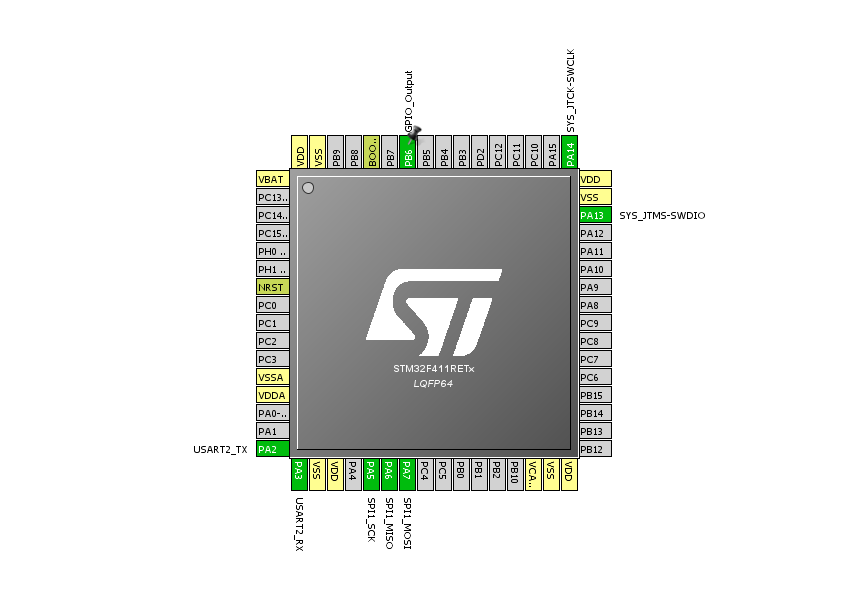
\includegraphics[width=400px]{img/cubemx.png}
    \caption{Praktinės dalies mikro-procesoriaus konfigūracija, naudojant STM32CubeMX \cite{STM3293:online}}
    \label{fig:stm32_cube_mx}
\end{figure}

Mikro-valdiklis sujungtas su jutikliu, naudojant SPI komunikacijos jungtį.
SPI jungtis reikalauja keturių jungčių -- laikrodžio (SCK), pasirinkimo (SS) ir dviejų duomenų linijų: MISO/MOSI.
MPU-9250 jutiklio specifikacijoje, šios kojos yra aprašomos kaip SCL, NCS, SDA ir AU0.
Iš paminėtų linijų, SCL jungiam prie SCK, NCS jungiam su SS, MISO jungiam su AU0 ir MOSI su SDA.
Tolimesnė SPI komunikacija yra vykdoma pagal protokolą.

Prieš pradedant bet kokių jutiklio duomenų nuskaitymą, būtina pasitikrinti ar komunikacija su jutikliu yra galima.
Tokiu tikslu jutikliui yra siunčiamas pasisveikinimo kodas -- \textit{0x75}.
Į kurį jutiklis turi atsakyti \textit{0x71}.
Jeigu atsakymas nėra toks -- vadinasi komunikacija nėra vykdoma ir jokie duomenų mainai nėra galimi.
Iš praktinės dalies galima paminėti, jog jeigu yra gaunamos kažkokios kraštutinės reikšmės -- \textit{0x00} arba \textit{0xFF}, SPI protokolo sujungimas visiškai nedirba ir problema tikrai bus arba litavime arba pačiuose kontaktuose, bet tikrai ne programinėje įrangoje.

Tolimesnis žingsnis yra normalizavimas.
Kiekvienas MPU-9250 yra normalizuojamas gamykloje, tačiau nėra pašalinama \textit{z} ašies gravitacinė komponentė.
Tai padaryta dėl to, kad skirtingose planetos vietose gravitacinė komponentė yra skirtinga, todėl jos normalizuoti nėra tikslo.
Kadangi vis tiek atliksime normalizavimą vienai ašiai -- galime iškarto normalizuoti ir likusias tris -- tiek linijinio, tiek kampinio pagreičio komponentes.

Normalizavimo proceso rezultatas yra nuolatinės dedamosios radimas.
Norint rasti nuolatinę dedamąja, reikia jutiklį paruošti -- jį korektiškai sukonfigūruoti, kad jis dirbtų prie savo galimų ribų.
Nustatyti žemo lygio filtrą iki $188 HZ$, pakelti mėginių rinkimo dažnį iki $1Khz$, kampinį pagreičio tikslumą nustatyti $250$ laipsnių per sekundę, o linijinį pagreičio tikslumą nustatyti $2g$.
Tuomet reikia surinkti pakankamą mėginių skaičių.
Skirtingi sprendimai renka skirtingus mėginių skaičių, todėl šiuo atveju bus pasirinkta $64$ mėginiai.
Tolimesnė eiga yra rasti visų mėginių vidurkį, pagal kiekvieną ašį.
Šitie skaičiai ir yra nuolatinės dedamosios komponentai. Juos reikia pašalinti iš gautų iš jutiklių duomenų.

Turint normalizuotus jutiklių duomenis, įmanomas duomenų rinkimas.


  \section{Modelio apibrėžimas}

  Norint atlikti filtravimo operaciją, reikalingas tam tikras modelis, kuriuo pagalba bus atliekama pati operacija.
Modelis apibūdina nagrinėjamą sistemą, kokios komponentės, kaip priklauso nuo esamų parametrų.
Visas žinias apie sistemą turi pateikti modelį kurianti pusė.

\subsection{Pradinis modelis}

Naudojamas jutiklis yra pagreičio jutiklis.
Pagreičio jutiklis grąžina momentinį pagreičio pokytį duotuoju matavimo gavimo metu, $a(t)$.
Tokių duomenų realus pavyzdys pateikiamas \ref{fig:ax_accel} pav.

Turėdami pagreičio duomenis, laiko momentu galima gauti greičio duomenis $v(t)$, \ref{fig:ax_velocity} pav.

\begin{equation}
    v(t) = \int_0^t a(t) \delta t
\end{equation}

Pozicijos pokytis $s(t)$ priklauso nuo objekto greičio $v(t)$, \ref{fig:ax_distance} pav.

\begin{equation}
    s(t) = \int_0^tv(t) \delta t
\end{equation}

Iš to seka, kad norint gauti sistemos poziciją, pagreitį reikia integruoti du kartus, \ref{fig:ax_distance} pav.

\begin{equation}
    s(t) = \int_0^tv(t) \delta t = \int_0^t \int_0^t a(t) \delta t \delta t
\end{equation}

\begin{figure}[b]
    \centering
    \caption{Vienos ašies pagreičio jutiklio matavimo duomenys}
    \label{fig:ax_accel}
    \begin{tikzpicture}
        \begin{axis}[
            width=400pt,
            height=150pt,
            xlabel={$t, s$},
            ylabel={$m/s^2$},
            grid=major
        ]
            \addplot[smooth] table [x index = {0}, y index = {1}, col sep=comma] {data/acceleration.csv};
        \end{axis}
    \end{tikzpicture}
\end{figure}

\begin{figure}
    \centering
    \caption{Greičio duomenys, gauti integruojant pagreičio jutiklio vienos ašies duomenis}
    \label{fig:ax_velocity}
    \begin{tikzpicture}
        \begin{axis}[
            width=400pt,
            height=150pt,
            xlabel={$t, s$},
            ylabel={$m/s$},
            grid=major
        ]
            \addplot[smooth] table [x index = {0}, y index = {2}, col sep=comma] {data/acceleration.csv};
        \end{axis}
    \end{tikzpicture}
\end{figure}

\begin{figure}
    \centering
    \caption{Atstumo duomenys, gauti integruojant greičio duomenis pagal \ref{fig:ax_velocity}}
    \label{fig:ax_distance}
    \begin{tikzpicture}
        \begin{axis}[
            width=400pt,
            height=150pt,
            xlabel={$t, s$},
            ylabel={$m$},
            grid=major
        ]
            \addplot[smooth] table [x index = {0}, y index = {3}, col sep=comma] {data/acceleration.csv};
        \end{axis}
    \end{tikzpicture}
\end{figure}

Tokiu būdu gaunamas paprasčiausias matematinis modelis, kurio pagalba galima nustatyti dabartinę objekto poziciją.
Didžiausias šito modelio trūkumas, kuris matosi ir pateiktuose \ref{fig:ax_accel}, \ref{fig:ax_velocity} ir \ref{fig:ax_distance} pavyzdžiuose, yra triukšmo dauginimas dėl dvigubo integravimo.
Pagreitis turi labai didelį matavimo triukšmą.
Integruojant vieną kartą, triukšmo įtaka matavimui yra padidinama du kartus.
Integruojant du kartus -- triukšmas padidėja keturis kartus.

\subsection{\textit{Kalman} filtro modelis}

\textit{Kalman} filtras reikalauja modelį aprašyti priklausomybės lygčių sistema.
Sistema turi apibūdinti gaunamų duomenų priklausomybę nuo galutinės sistemos būsenos.
Aprašymas pradedamas nuo pagreičio matavimo matmens

\begin{equation}
    a(t) = a(t)
\end{equation}

Greitis priklauso nuo greičio, kuris buvo vienu laiko momentu prieš, ir nauju pagreičiu

\begin{equation}
    v(t) = v(t-1) + a(t) * \delta t
\end{equation}

Pozicija priklauso nuo prieš tai buvusios pozicijos, dabartinio greičio poslinkio, bei pagreičio kvadrato

\begin{equation}
    s(t) = s(t-1) + v(t-1) + \frac{a(t)}{2}\delta t^2
\end{equation}

Iš šitų lygčių yra sudaromas sistemos būsenos modelis

\begin{equation}
    \hat{x} = \begin{cases}
        s(t-1) + v(t-1) + \frac{a(t)}{2}\delta t^2 \\
        v(t-1) + a(t) * \delta t \\
        a(t)
    \end{cases}
\end{equation}

Kadangi iš viso mes turime tris ašis, modelis patrigubėja ir iš viso jį sudaro

\begin{equation}
    \hat{x} = [ x, y, z, \dot{x}, \dot{y}, \dot{z}, \ddot{x}, \ddot{y}, \ddot{z}]^T,
\end{equation}
kur $\dot{x}$ yra pozicijos pirmą išvestinė -- greitis, $\ddot{x}$ yra pozicijos antra išvestinė -- pagreitis.

Galutinė sistemos būsenos matrica atrodo

\begin{equation}
    F = \begin{bmatrix}
        1 & 0 & 0 & dT & 0 & 0 & 0.5*dT^2 & 0 & 0 \\
        0 & 1 & 0 & 0 & dT & 0 & 0 & 0.5*dT^2 & 0 \\
        0 & 0 & 1 & 0 & 0 & dT & 0 & 0 & 0.5*dT^2 \\
        0 & 0 & 0 & 1 & 0 & 0 & -dT & 0 & 0 \\
        0 & 0 & 0 & 0 & 1 & 0 & 0 & -dT & 0 \\
        0 & 0 & 0 & 0 & 0 & 1 & 0 & 0 & -dT \\
        0 & 0 & 0 & 0 & 0 & 0 & 1 & 0 & 0 \\
        0 & 0 & 0 & 0 & 0 & 0 & 0 & 1 & 0 \\
        0 & 0 & 0 & 0 & 0 & 0 & 0 & 0 & 1
    \end{bmatrix},
\end{equation}
kur $dT$ yra laikas, nusakantis kaip dažnai buvo daromi matavimai.

\textit{Kalman} filtro veikimui yra reikalauja turėti matavimų matricą.
Matavimų matrica nurodo, kuris iš modelio komponentų yra pats matavimas.
Šiuo atveju egzistuoja trys pagreičio komponentės, kurios nusako atliekamus matavimus.

\begin{equation}
    H = \begin{bmatrix}
        1 & 0 & 0 & 0 & 0 & 0 & 0 & 0 & 0 \\
        0 & 1 & 0 & 0 & 0 & 0 & 0 & 0 & 0 \\
        0 & 0 & 1 & 0 & 0 & 0 & 0 & 0 & 0
    \end{bmatrix}
\end{equation}

Pasirinkus matavimo matrica, toliau reikia pasirinkti dvi triukšmo įverčius.
Pirmas įvertis $q$, kuris nusako \textit{Kalman} filtro darbo proceso triukšmą.
Antras įvertis $r$ yra matavimo triukšmas. 
Matavimo triukšmo įvertį galima nustatyti dviem keliais. 
Pirmas kelias yra eksperimentinis -- atlikti stabilios matavimus ant stabilios platformos ir panaudoti gautą nuokrypį kaip matavimo triukšmą.
Kitas kelias yra pasikliauti gamintojo nurodytu matavimo skaičiumi.
Proceso triukšmas modelyje šiuo atveju yra pasirenkamas lygus matavimo triukšmui modelio paprastumui ir jie abu yra lygus $0.1$.

Turint modelio lygčių sistemą, matavimo matricą bei triukšmus, galima pradėti dirbi su \textit{Kalman} filtru.
Norint teisingai įvertinti \textit{Kalman} filtro darbą su duomenimis, visi įėjimo duomenys yra modeliuojami paprastu $sin$ signalu, pridedant atsitiktinį baltąjį triukšmą.
Signalo pavyzdys pateikiamas \ref{fig:sin_acc_data_with_noise} pav.
Kaip matosi iš grafiko, signalas pats turi labai daug triukšmo, tačiau seka labai specifinį kelią, kurį galima atsekti su paprastu vidurkinimu.
Toks signalas nėra pilnai atsitiktinis, jis turi kažkokį dėsnį.
Atlikus dvigubą originalaus signalo integravimą, gaunamas atstumo pokytis \ref{fig:sin_distance_data_with_noise} pav.
Tiesinį \textit{Kalman} filtro modelio rezultatas bus lyginamas su šiuo rezultatu ir bus laikomas teisingo rezultato etalonas.

\begin{figure}
    \centering
    \caption{Palyginimui naudojamas $sin$ signalas, su pridėtu baltuoju triukšmu}
    \label{fig:sin_acc_data_with_noise}
    \begin{tikzpicture}
        \begin{axis}[
            width=300pt,
            height=150pt,
            xlabel={$t, s$},
            ylabel={$m/s^2$},
            grid=major
        ]
            \addplot[smooth] table [x index = {0}, y index = {1}, col sep=comma] {data/linear_kalman.csv};
        \end{axis}
    \end{tikzpicture}
\end{figure}

\begin{figure}
    \centering
    \caption{Atstumo pokytis, dvigubai integruojant $sin$ signalą}
    \label{fig:sin_distance_data_with_noise}
    \begin{tikzpicture}
        \begin{axis}[
            width=300pt,
            height=150pt,
            xlabel={$t, s$},
            ylabel={$m$},
            grid=major
        ]
            \addplot[smooth] table [x index = {0}, y index = {3}, col sep=comma] {data/linear_kalman.csv};
        \end{axis}
    \end{tikzpicture}
\end{figure}

Pateikus į tiesinį \textit{Kalman} filtrą duomenis, kuris remiasi ankščiau aprašytomis lygtimis, gaunamas rezultatas, kuris yra pateikiamas \ref{fig:linear_kalman_filter_sin} pav.
Duotas grafikas pateikia esminį tiesinio \textit{Kalman} filtro naudojimo trūkumą duotos problemos atveju.
Esami duomenys visiškai neturi jokio tiesinės interpretacijos, todėl tiesinis \textit{Kalman} filtras šiuo atveju nėra tinkamas.
Reikia panaudoti tokį sprendimą, kurį galima būtų pritaikyti ne tiesinėms sistemoms.

\begin{figure}
    \centering
    \caption{Tiesinio Kalman filtro pozicijos pokyčio rezultatas, lyginant su pradiniais duomenimis}
    \label{fig:linear_kalman_filter_sin}
    \begin{tikzpicture}
        \begin{axis}[
            width=300pt,
            height=150pt,
            xlabel={$t, s$},
            ylabel={$m$},
            grid=major,
            legend pos=outer north east
        ]
            \addplot[smooth, dashed] table [x index = {0}, y index = {3}, col sep=comma] {data/linear_kalman.csv};
            \addplot[smooth] table [x index = {0}, y index = {4}, col sep=comma] {data/linear_kalman.csv};
            \legend{Pradinis pokytis, Tiesinio filtro pokytis}
        \end{axis}
    \end{tikzpicture}
\end{figure}

\subsection{Išplėstasis \textit{Kalman} filtras}

Išplėstasis \textit{Kalman} filtras yra netiesinis \textit{Kalman} filtras.
Tai yra pasiekiama, panaudojus \textit{Jacobian} matricą, kurios pagalba ne tiesinė lygtis yra ištiesinama viename taške.

Modelis, kuris yra pateikiamas išplėstajam \textit{Kalman} filtrui turi būti ne matricinės, o lygčių sistemos formos, kadangi bus atliekamas diferencialinis skaičiavimas.
Dėl šitos priežasties, nagrinėjamas modelis yra perrašomas į lygčių sistemą

\begin{equation}
    \hat{x} = \begin{cases}
        x_1 + x_2 + x_3 * 0.5 * dT^2 \\
        x_2 + x_3 * dT \\
        x_3
    \end{cases}
\end{equation}

Toliau reikia perrašyti matavimo gavimo matricą į lygtį.
Kadangi matavimas yra gaunamas tiesiogiai, tai ir pati lygtis yra tiesinė lygtis

\begin{equation}
    h(\hat{x}) = x_3;
\end{equation}

Sekantis žingsnis yra nustatyti triukšmus.
Norint palyginti išplėstąjį \textit{Kalman} filtro modelį su tiesiniu \textit{Kalman} filtro modeliu, pasirenkamos tokie patys triukšmų įverčiai.

Pateikus tokius pačius duomenis, kaip ir į tiesinį \textit{Kalman} filtrą, išplėstinio \textit{Kalman} filtro rezultatas yra pateikiamas \ref{fig:extended_kalman_filter_sin} pav.

\begin{figure}
    \centering
    \caption{Išplėsto Kalman filtro pozicijos pokyčio rezultatas, lyginant su pradiniais duomenimis}
    \label{fig:extended_kalman_filter_sin}
    \begin{tikzpicture}
        \begin{axis}[
            width=300pt,
            height=150pt,
            xlabel={$t, s$},
            ylabel={$m$},
            grid=major,
            legend pos=outer north east
        ]
            \addplot[smooth, dashed] table [x index = {0}, y index = {1}, col sep=comma] {data/extended_kalman.csv};
            \addplot[smooth] table [x index = {0}, y index = {2}, col sep=comma] {data/extended_kalman.csv};
            \legend{Pradinis pokytis, Išplėsto filtro pokytis}
        \end{axis}
    \end{tikzpicture}
\end{figure}

Lyginant tiesinio \textit{Kalman} filtro \ref{fig:linear_kalman_filter_sin} rezultato ir išplėstojo \textit{Kalman} filtro rezultato \ref{fig:extended_kalman_filter_sin} grafikus, galima teigti, jog išplėstasis \textit{Kalman} filtras veikia geriau.
Tai yra logiškas ir lauktas rezultatas, kadangi išplėstasis \textit{Kalman} filtras yra skirtas dirbti su ne tiesinėmis sistemomis \cite{6851407}.
Šiuo atveju, uždaviniui spręsti galima pasirinkti išplėstąjį \textit{Kalman} filtrą, tačiau tai yra ne paskutinis galimas problemos sprendimo būdas.
Šiuo metu labai pradeda populiarėti sekamasis \textit{Kalman} filtras, kuris sprendžia vieną pagrindinių išplėstojo \textit{Kalman} filtro problemų -- tiesinimo triukšmą.

\subsection{Sekamasis \textit{Kalman} filtras}

Sekamasis \textit{Kalman} filtro modelio reikalavimai yra lygiai tokie patys, kaip išplėstojo \textit{Kalman} filtro, todėl modelio perrašinėti nėra tikslo.
Triukšmo įverčiai yra paliekami tokie patys, kaip ir tiesinio bei išplėstinio filtro atvejais.
Modelio veikimo rezultatas yra pateikiamas \ref{fig:unscented_kalman_filter_sin} pav.

\begin{figure}
    \centering
    \caption{Sekamojo \textit{Kalman} filtro pozicijos pokyčio rezultatas, lyginant su pradiniais duomenimis}
    \label{fig:unscented_kalman_filter_sin}
    \begin{tikzpicture}
        \begin{axis}[
            width=300pt,
            height=150pt,
            xlabel={$t, s$},
            ylabel={$m$},
            grid=major,
            legend pos=outer north east
        ]
            \addplot[smooth, dashed] table [x index = {0}, y index = {1}, col sep=comma] {data/unscented_kalman.csv};
            \addplot[smooth] table [x index = {0}, y index = {2}, col sep=comma] {data/unscented_kalman.csv};
            \legend{Pradinis pokytis, Sekamo filtro pokytis}
        \end{axis}
    \end{tikzpicture}
\end{figure}

\subsection{Modelio pasirinkimas}

Sekamasis \textit{Kalman} filtras \ref{fig:unscented_kalman_filter_sin}, lyginant su išplėstuoju \textit{Kalman} filtru \ref{fig:extended_kalman_filter_sin} grafiškai neturi didelių privalumų.
Rezultato grafikas atrodo beveik identiškai.
Skirtumas matosi įverčiams artėjant prie nulinio pozicijos pokyčio, laiko momentu $t=6s$.
Išplėstasis Kalman filtras toje srityje turi pokytį tarp realios reikšmės ir filtruotos reikšmės, tuo tarpu sekamasis \textit{Kalman} filtras priartėja prie realios reikšmės, ko pasekoje mažina klaidos vertę.

Norint išmatuoti skaitinėmis reikšmėmis šių trijų pateiktų filtrų tikslumų skirtumus, bus panaudota kryžminė koreliacija.
Kryžminė koreliacija yra plačiai naudojamas matas, nustatyti panašumus tarp dviejų signalų.
Kuo gautas skaitinis įvertis yra arčiau nulio -- tuo signalai yra panašesni.
Verta paminėti, kad šitas matavimas yra naudojamas metodų palyginimui.

\begin{table}
    \centering
    \caption{Kryžminės koreliacijos matavimo rezultatas kiekvienam filtrui}
    \label{table:kalman_filter_comparison}
    \begin{tabular}{|c|c|c|} \hline
        Filtras & Koreliacija \\ \hline
        Tiesinis Kalman filtras & 0.8811 \\ \hline
        Išplėstas Kalman filtras & 0.9989 \\ \hline
        Sekamas Kalman filtras & 1.0000 \\ \hline
    \end{tabular}
\end{table}

Pagal gautus duomenis, kurie yra pateikiami \ref{table:kalman_filter_comparison} lentelėje galima daryti išvadas, kad geriausiai duomenis filtruoja būtent sekamasis \textit{Kalman} filtras ir netoli jo yra išplėstasis \textit{Kalman} filtras.
Remiantis šiuo rezultatu, filtro įgyvendinimui yra pasirenkamas sekamasis \textit{Kalman} filtras.

\subsection{Išvados}

Šiame skyriuje buvo apžvelgti trys filtro modeliai -- tiesinis, išplėstasis ir sekamasis \textit{Kalman} filtrai.
Palyginimas pradėtas nuo tiesioginio signalo dvigubo integravimo matavimo, kuris iš pirminės grafinės signalo analizės buvo nustatytas visiškai nepanaudojamas.
Pirmas realus nagrinėjamas paprastas \textit{Kalman} filtras, kuris reikalauja apibrėžti sistema lygčių sistema.
Tai yra žinios iš išorės, kuris yra reikalingos teisingai suderinti \textit{Kalman} filtro darbą.
Norint patikrinti \textit{Kalman} filtro veikimą, reikia į jį paduoti duomenis, kurių teisingas rezultatas yra iš anksto žinomas.
Dėl šios priežasties buvo pasirinktas paprastas sinuso tipo pagreičio signalas ir prie jo pridėtas baltasis triukšmas.
Tokiu būdu yra generuojamas signalas, kurio rezultatas yra iš anksto žinomas ir taip galima vertinti filtro darbą.
Atliktas matavimas parodė, kad tiesinis \textit{Kalman} filtras yra visiškai netinkamas darbo uždaviniui spręsti.
Sekantys du filtrai sprendžia paprasto \textit{Kalman} filtro pagrindinę problemą -- sistema turi būtinai būti tiesinė: išplėstas ir sekamasis \textit{Kalman} filtras.
Išplėstasis \textit{Kalman} filtras yra labai paplitęs filtras navigacinėse sistemose, todėl jis ir buvo pasirinktas kaip pirmas filtras, kuris sugeba dirbti su netiesine sistema.
Matavimas su žinomais duomenimis parodė, kad jis dirba geriau už paprastą \textit{Kalman} filtrą.
Sekamasis \textit{Kalman} filtras yra naujas filtro tipas, kuris po truputi įgauna populiarumą.
Jo matavimas parodė, kad jis veikia geriau už išplėstąjį \textit{Kalman} filtrą.
Dėl šios priežasties pasirenkamas sekamasis \textit{Kalman} filtras.




  \section{Įgyvendinimas}

  Nustačius tinkamiausią modelį, jį reikia perkelti į įterptinę sistemą.
Darbui yra panaudota \textit{STM32f411RE} vystymo plokštė, kuri buvo apžvelgta \ref{hardware} skyriuje.
Viso algoritmo veikimo blokinė schema yra pateikta \ref{subsection:2_priedas} priede.

\subsection{Modelis}

Darbo patogumui modelis yra aprašomas \ref{code:kalman_model_struct} programiniam kode pateikiama struktūra. 
Tai leidžia izoliuoti filtro modelio parametrus nuo globalių ir lokalių kintamųjų ir per vieną struktūros kintamąjį pasiekti visus reikalingus modelio parametrus.
Struktūroje dominuoja du tipai parametrų \textit{arm\_matrix\_instance\_f32} ir \textit{float32\_t}.
Pirmas tipas yra skirtas darbui su matrica.
Tai yra specialus duomenų tipas, kuris skirtas darbui su ,,Cortex-M4'' šeimos procesorių matematine posisteme.
Jis yra \textit{struct} tipo kintamasis, kuris aprašo tris kintamuosius - matricos eilučių, stulpelių skaičių ir nuorodą į \textit{float32\_t} tipo masyvą.
Verta pastebėti, kad struktūroje beveik kiekvienas iš \textit{arm\_matrix\_instance\_f32} tipo kintamųjų turi ir \textit{float32\_t} tipo aprašus, kurie bus atitinkamai sujungti.
Taip yra daroma, kad deklaruojant kelis modelius, jų kintamieji būtų deklaruojami iš naujo ir atmintyje būtų saugomi atskirai.

Toliau seka modelio pradinių parametrų suteikimas.
Šis žingsnis yra atliekamas tam, kiekvienas iš struktūroje aprašytų parametrų įgautų realią vertę arba nuorodą į realią vertę.
Visi \textit{arm\_matrix\_instance\_f32} tipo kintamieji yra inicijuojami vienodai, naudojant \textit{arm\_mat\_init\_f32} metodą.
Kodo pavyzdys yra pateikiamas \ref{code:arm_matrix_init} programiniam kode.
Pirmas metodo argumentas yra \textit{arm\_matrix\_instance\_f32} kintamojo nuoroda, antras argumentas yra eilučių skaičius, trečias argumentas yra stulpelių skaičius, ketvirtas argumentas yra slankaus kablelio masyvo kintamasis, kurio nuoroda bus priskiriama pirmo argumento matricai.

\begin{cfigure}[b]
    \centering
    \caption{Arm matricos kintamojo tipo inicijavimas}
    \label{code:arm_matrix_init}
    \begin{lstlisting}
arm_mat_init_f32(&m->f, 3, 3, (float32_t *)f_f32);
    \end{lstlisting}
\end{cfigure}

Proceso triukšmas pasirenkamas $q = 0.1$, dėl to proceso matrica, inicijavimo metu, yra aprašoma \ref{code:arm_q_matrix_init} programiniu kodu.
Reikalinga yra įstrižainė matrica, kurios dydis yra 3 eilutės ir 3 stulpeliai, todėl triukšmo įverčiai yra priskiriami $0$, $4$ ir $8$ masyvo vietoms.
Matavimo triukšmui inicijuoti yra taikoma lygiai tokia pati procedūra, tik šiuo atveju kintamasis yra vieno skaičiaus dydžio ir deklaruojama matrica yra $1x1$.
Paskutiniai inicijuojami parametrai yra $MM$ ir $PP$.
Parametras $MM$ yra naudojamas saugoti naujausią filtro vidurkio sprendinį.
Šį parametrą pirmu darbo ciklu suteiks pats filtras, todėl visi šios matricos įverčiai turi būti $0$.
Parametras $PP$ yra naudojamas saugoti naujausią filtro kovariacijos sprendinį.
Jis yra inicijuojamas su parametru $0.1$.
Antru darbo ciklu filtras atnaujins įvertį.
Šiuo žingsniu filtro modelio inicijavimas yra baigiamas.
Toliau reikia įgyvendinti patį sekamą Kalman filtrą.

\begin{cfigure}
  \centering
  \caption{Kalman modelio struktūra}
  \label{code:kalman_model_struct}
  \begin{lstlisting}
typedef struct KModel {
    arm_matrix_instance_f32 f;
    arm_matrix_instance_f32 h;
    float32_t dT;
    uint8_t n;
    uint8_t ss;
    float32_t q;
    float32_t r;
    float32_t Q_f32[9];
    arm_matrix_instance_f32 Q;
    float32_t R_f32[1];
    arm_matrix_instance_f32 R;
    uint8_t kappa;
    float32_t W_f32[7];
    arm_matrix_instance_f32 W;
    float32_t c;
    float32_t MM_f32[3];
    arm_matrix_instance_f32 MM;
    float32_t PP_f32[9];
    arm_matrix_instance_f32 PP;
} KModel;
  \end{lstlisting}
\end{cfigure}


\subsection{Filtras}

Filtro darbas yra pradedamas nuo sigma taškų skaičiavimo.
Sigma taškų skaičiavimams atlikti. jie yra perkeliami į atskirą funkciją, kuri priimta keturis argumentus.
Pirmas argumentas yra vidurkio matrica, antras argumentas yra kovariacijos matrica, trečias argumentas yra $c$ konstanta ir paskutinis argumentas yra matrica, į kurią bus įrašomi gauti sigma taškai.
Sigma taškų skaičiavimas susideda iš trijų žingsnių:

\begin{enumerate}
    \item apskaičiuoti \textit{Cholesky} dekompoziciją;
    \item atlikti aritmetines operacijas su gautomis vertėmis iš dekompozicijos;
    \item sujungti gautus rezultatus į vieną matricą;
\end{enumerate}

\begin{cfigure}
    \centering
    \caption{Proceso triukšmo matricos inicijavimas}
    \label{code:arm_q_matrix_init}
    \begin{lstlisting}
m->Q_f32[0] = 0.01;
m->Q_f32[4] = 0.01;
m->Q_f32[8] = 0.01;

arm_mat_init_f32(&m->Q, 3, 3, m->Q_f32);
    \end{lstlisting}
\end{cfigure}

Reikalingos \textit{Cholesky} dekompozicijos įgyvendinimas taip pat yra iškeliamas į kitą funkciją, kuri turi tris argumentus -- matricą, kurią riekia transformuoti, dimensijų skaičių ir išėjimo matricą.
Dekompozicijos įgyvendinimas yra skolinamas iš \cite{Cholesky6:online}.
Gautą dekompozicijos rezultatą reikia padauginti iš konstantos.
Tai atlikti yra labai lengva, panaudojus \textit{cortex} skaičiavimo posistemes siūlomomis funkcijomis.
Kodo pavyzdys yra pateikiamas \ref{code:arm_mat_scale_P} programiniame kode.
Pirmas metodo argumentas yra pradinė matrica, antras argumentas yra konstanta, trečias argumentas yra galutinė matrica.

\begin{cfigure}
    \centering
    \caption{Matricos dauginimas iš konstantos}
    \label{code:arm_mat_scale_P}
    \begin{lstlisting}
arm_mat_scale_f32(&Pc, c, &A);
    \end{lstlisting}
\end{cfigure}

Toliau reikia atlikti sudėties ir atminties operacijas su matricomis.
Pirma matrica yra gauto vidurkių vektoriaus pakartojimas iki simetrinės matricos.
Ši matrica bus saugoma $Y$ nuorodoje.
Šis tikslas yra pasiekiamas panaudojus \textit{arm\_mat\_sub\_f32} ir \textit{arm\_mat\_add\_f32} funkcijas.
Paskutinė operacija yra sujungti gautus rezultatus į vieną matricą.
Pirmas stulpelis yra įėjimo vidurkiai, nuo antro iki ketvirto yra $Y+A$ ir nuo penkto iki septinto $Y-A$.
Taip yra gaunama išvedimo matrica.

Turint sigma taškus, toliau reikia juos transformuoti.
Transformacija \cite{julier2002scaled} yra vadinama \textit{Unscented transformation}.
Ši transformacija leidžia gauti tiesinę sistemą.
Transformacija yra aprašoma atskiroje funkcijoje.
Priimami įėjimo parametrai -- netiesinė perdavimo funkcija, sigma taškai, vidurkių taškų svoriai, kovariacija.
Išėjimo parametrai yra transformuotas vidurkis, taškai, kovariacija ir nukrypimas.
Spėjimo žingsnyje, perdavimo funkcija yra modelio netiesinė funkcija, sigma taškai yra sigma taškai, gauti iš sigma taškų generavimo, o kovariacija yra sistemos triukšmo matrica.
Transformacija yra atliekama nuosekliai per stulpelį.
Gauti sigma taškai yra paduodami į netiesinę perdavimo funkciją, gautas rezultatas (transformuoti taškai) padauginamas iš to stulpelio svorio ir gautas įvertis yra sumuojamas (\ref{code:arm_mean_and_poin_transformation} programinis kodas).
Tokiu būdu yra gaunamas transformuotas vidurkis.
Transformuotas nukrypimas yra skaičiuojamas atimant kiekvieną transformuotų taškų stulpelį iš transformuotų vidurkių vektoriaus.
Kovariacija yra gaunama padauginus nuokrypį iš svorių įstrižainės matricos. Šia skaičiavimų seka baigiamas spėjimo filtro žingsnis.
Tolimesnis kodas yra skirtas filtro koregavimui.

\begin{cfigure}
    \centering
    \caption{Taškų ir vidurkio transformavimas}
    \label{code:arm_mean_and_poin_transformation}
    \begin{lstlisting}
// copy i-th column from X to X_temp_f32
for (ut_i_i = 0; ut_i_i < X->numRows; ut_i_i++) {
    uint8_t ut_i_i_ind = ut_i_i * X->numCols+ut_i;
    X_temp_f32[ut_i_i] = X->pData[ut_i_i_ind];
}

arm_mat_init_f32(&X_temp, 3, 1, X_temp_f32);
arm_mat_mult_f32(f, &X_temp, &Y_temp);

for (ut_j = 0; ut_j < 3; ut_j++) {
    uint8_t ut_y_ind = (ut_j*7)+ut_i;
    Y->pData[ut_y_ind] = Y_temp.pData[ut_j];
}

// multiply W(k)*Y(:,k);
arm_mat_scale_f32(&Y_temp, W->pData[ut_i], &y_temp_2);
// y + W(k)*Y(:,k)
arm_mat_add_f32(&y_temp, &y_temp_2, &y_temp);
    \end{lstlisting}
\end{cfigure}

Filtro koregavimas yra pradedamas nuo matavimo perdavimo funkcijos tiesinimo operacijos, panaudojus tą pačią transformaciją, kuri buvo panaudota ir spėjimo žingsnyje.
Šiuo atveju perdavimo funkcija yra matavimo funkcija, sigma taškai yra jau transformuoti sigma taškai, kurie yra gaunami iš spėjimo žingsnio transformacijos, o kovariacijos matrica yra matavimo triukšmo matrica.
Sekantis žingsnis yra Kalman filtro įverčio skaičiavimas.
Reikia pradėti nuo jungtinį sistemos ir matavimo kovariacijos transformacijos vertės skaičiavimo.
Toliau reikia sudėti matavimo triukšmą su transformuota matavimo kovariacija.
Turint šituos du įverčius, juos reikia padalinti vieną iš kito ir taip yra gaunamas Kalman filtro įvertis matricos formoje (\ref{code:arm_kalman_gain_calculation} programinis kodas).

\begin{cfigure}
    \centering
    \caption{Kalman filtro įverčio skaičiavimas}
    \label{code:arm_kalman_gain_calculation}
    \begin{lstlisting}
// P_xz = X_dev * diag(W) * Z_dev';
arm_mat_mult_f32(&X_dev, &W_diag, &X_dev_W_diag);
arm_mat_trans_f32(&Z_dev, &Z_dev_transpose);
arm_mat_mult_f32(&X_dev_W_diag, &Z_dev_transpose, &P_xz);
// S = R + P_zz;
arm_mat_add_f32(&model->R, &P_zz, &S);
// K = P_xz / S;
arm_mat_inverse_f32(&S, &S_inv);
arm_mat_mult_f32(&P_xz, &S_inv, &K);
    \end{lstlisting}
\end{cfigure}

Turint Kalman filtro matricą, galima atnaujinti spėjamus parametrus.
Kalman filtro matrica yra dauginama iš matavimo įverčio ir transformuoto matavimo įverčio skirtumo.
Spėjamas vidurkis yra gaunamas sudedant transformuotą vidurkį ir prieš tai aprašytą sandaugą.
Kovariacija gaunama sudauginus junginę kovariaciją su Kalman filtro matrica.
Su gauta matrica yra skaičiuojamas skirtumas tarp spėjimo metu transformuota kovariacija (\ref{code:arm_kalman_measurement_update} pav.).

\begin{cfigure}
    \centering
    \caption{Vidurkio ir kovariacijos atnaujinimas}
    \label{code:arm_kalman_measurement_update}
    \begin{lstlisting}
// m = m_hat + K *(Z_r - z_hat);
arm_mat_sub_f32(&Z_r, &z_hat, &Z_r_z_hat);
arm_mat_mult_f32(&K, &Z_r_z_hat, &K_Z_r_z_hat);
arm_mat_add_f32(&m_hat, &K_Z_r_z_hat, &model->MM);

// P = P_hat - P_xz * K';
arm_mat_trans_f32(&K, &K_transpose);
arm_mat_mult_f32(&P_xz, &K_transpose, &P_xz_K_transpose);
arm_mat_sub_f32(&P_hat, &P_xz_K_transpose, &model->PP);
    \end{lstlisting}
\end{cfigure}

\subsection{Išvados}

Įgyvendinimo metu buvo iškilę porą sunkumų.
Vienas iš sunkumų yra paprastų duomenų perkėlimo operacijų su matricomis nebūvimas.
Jeigu reikia išplėsti $3x1$ vektorių į $3x3$ matrica, kur kiekvienas stulpelis yra pirmo stulpelio kartotinis, šią operaciją reikia rašyti savarankiškai.
Dėl šios priežasties gali atsirasi klaidos sistemos veikime ir reikia praleisti daug laiko įsitikinant, kad parašyta funkcija veikia gerai.
Tuo tarp tarpu, darbo su matricomis programiniam pakete, tokią operaciją yra labai lengva parašyti, kadangi pats programinis paketas jau turi įgyvendinęs šitą operaciją.
Dar viena didelę problema yra sudėtingų algoritmų įgyvendinimas.
Šiuo atveju, darbe buvo reikalinga \textit{Cholesky} dekompozicija.
Internete rastas algoritmo įgyvendinimas negarantuoja, kad jis veikia lygiai taip pat, kaip ir matematiniam programiniam pakete pateiktas įgyvendinimas.
Nurodytas skirtumas galėjo pridėti papildomų įgyvendinimo kaštų.

Kitas didelis sunkumas yra kodo skaitymas.
Darbe su bet kokiu matematiniu programiniu paketu visos operacijos atrodo lengvai suprantamos, kadangi yra naudojami tie patys simboliai operacijoms pažymėti, kaip ir matematikos knygose.
Įgyvendinant matematines operacijas įterptinėje sistemoje, operacijos su matricomis tampa ne tokios lengvos skaityti.
Vietoj įprastų sumos ir daugybos ženklų atsiranda funkcijų kvietimas.
Dviejų matricų daugybą tampa trys funkcijų kvietimai ir dar porą pagalbinių matricų, kurių tikslas yra saugoti laikinus rezultatus.
Rašyti laikiną rezultatą į kažkokį realų kintamąjį yra labai rizikinga, kadangi tokia operacija kaip transponavimas gali būti atlikta neteisingai.

Paskutinis sunkumas yra atminties valdymas.
Darbo metu buvo panaudota pora operacijų, kurių tikslas yra atlikti duomenų kopijavimą iš vieno masyvo į kitą.
Tai sukėlė darbo su atmintimis problemas.
Kintamieji, su kuriais nebuvo daromos jokio operacijos gaudavo reikšmes, kurios neturėjo visiškai jokios prasmės.
Surasti iš ištaisyti tokio tipo klaidas yra be galo sudėtinga ir užima labai daug laiko kaštų.
Atliekant šitą darbą be skaičiavimo realizacijos reikia taip pat galvoti ir apie atminties naudojimo logiką.
Ar galima matricą pateikti kaip nekintančią ir taip sutaupyti darbinės atminties, panaudojus tik skaitymui skirtą atmintį.

Sekamo Kalman filtro perkėlimo į įterptinę sistemą metu, buvo parašyta iš viso 1636 eilutės kodo.







  \newpage

  \section*{Išvados}
  \addcontentsline{toc}{section}{Išvados}

  Žinių išgavimas yra procesas, kurio tikslas yra išgauti įdomius duomenų modelius iš didelio kiekio duomenų.
Tai taip pat yra vadinama žinių atradimo procesu ir jis tipiškai susideda iš duomenų valymo, integravimo, išrinkimo, transformavimo, modelio sukūrimo, jo įvertinimo ir gautų žinių atvaizdavimo.

Duomenų modelis yra įdomus jeigu jis galioja panaudojus testinius duomenis su tam tikru pasikliovimo lygiu, neįprastas ir potencialiai yra pritaikomas, paprastas suprasti žmogui.
Įdomūs duomenų modeliai sudaro žinias. 

Žinių inžinerija yra daugelio dimensijų požiūris į duomenis. Pagrindinės dimensijos yra duomenys, žinios, technologijos ir programos.

Žinių išgavimas gali būti suburtas iš skirtingo tipo duomenų, tol ko duomenis turi prasmę norimai sričiai, kaip duomenų bazės duomenis, duomenų saugyklos duomenis, perdavimo duomenis, ir pažengę duomenų tipai. 
Pažengę duomenų tipai susideda iš laikinės ar sekos duomenis, duomenų srautas, tūrinė informacija, tekstas ir daugialypės terpės duomenis, grafų ir tinklo duomenis.

Duomenų saugykla yra vieta saugoti duomenis ilgam laikotarpiui iš skirtingų šaltinų, bendroje schemoje.
Saugyklos sistemos pateikia daugelio dimensijų duomenis su analizės palaikymu, taip pat vadinamai realaus laiko analizės apdorojimui.

Daugelio dimensijų žinių išgavimas, integruoja pagrindinius žinių išgavimo metodus su realaus laiko daugelio dimensijų analize.
Metodas ieško įdomių modelių per skirtingas ir įvairias duomenų kombinacijas per skirtingas dimensijas, taikant skirtingas abstrakcijas, taip labai giliai analizuojant sąryšius tarp skirtingų dimensijų.

Žinių išgavimo funkcionalumai yra naudojami aprašant modelio arba žinių tipus, kurie buvo rasti per žinių išgavimą.
Tokie funkcionalumai yra charakterizavimas ir diskriminavimas, dažninių modelių išgavimas, asociacija ir koreliacija, klasifikavimas ir regresija, grupinė analizė; išskirčių aptikimas.

Žinių išgavimas turi labai daug pasisekusių įgyvendinimų, verslo srityje, interneto paieškoje, biologijos, sveikatos informatikoje, finansų, bibliotekos ir vyriausybės srityje.

  \newpage

  \addcontentsline{toc}{section}{Literatūra}

  \bibliographystyle{apa}
  \bibliography{references}

\end{document}
